\documentclass[12pt]{article}

\usepackage[T2A,T1]{fontenc}
\usepackage[utf8]{inputenc}
\usepackage[macedonian]{babel}
\usepackage{microtype}
\usepackage{amsmath,amssymb}
\microtypesetup{expansion=false}
\usepackage{csquotes}
\usepackage[hidelinks]{hyperref}
\usepackage{graphicx}
\usepackage{booktabs}
\usepackage{siunitx}

\title{Прогностичко моделирање на преживувањето кај рак на дојка}
\date{}

\begin{document}

\maketitle

\begin{abstract}
Оваа дипломска работа споредува модели за прогноза на преживувањето кај рак на
дојка во клиничката METABRIC кохорта. Cox PH, Баесови Weibull AFT и Random
Survival Forest (RSF) се оценети со клинички предиктори и со истите предиктори
дополнети со категоријалниот PAM50 подтип. Disease-specific survival (DSS) е
примарен исход, а overall survival (OS) е анализа на чувствителност. Аналитичката
кохорта има 1.979 пациентки и се дели еднаш на тренинг, калибрациски и тест-сет
со големини 989/495/495. Дискриминацијата, веројатносната точност и Баесовата
неизвесност се разгледуваат одделно. Клиничките модели имаат умерена и слична
DSS дискриминација, без стабилен победник низ метриките. PAM50 дава мали,
модел-зависни добивки: најдоследни кај RSF, ограничени кај Cox, а кај Weibull
најјасни за Uno C. Weibull fit-овите ги исполнуваат MCMC праговите, но posterior
predictive проверките и Weibull--lognormal разликите ја ограничуваат сигурноста
за моделската форма. За цензурирани исходи се применува конзервативна
split-conformal score-envelope постапка за ограниченото време. Набљудуваните
граници на покриеност се над номиналното ниво во оваа поделба, но медијаната на
ширината е околу 94 месеци при хоризонт од 120 месеци и 271--274 месеци при 300
месеци. Затоа покриеноста не подразбира доволна практична прецизност. DSS се
толкува како net survival под цензурирачки претпоставки, а резултатите не се
надворешна клиничка валидација.

\medskip
\noindent\textbf{Клучни зборови:} рак на дојка; METABRIC; анализа на
преживување; цензурирање; Weibull AFT; PAM50; conformal prediction.
\end{abstract}

\clearpage
\setcounter{tocdepth}{2}
\tableofcontents
\clearpage

\section{Вовед и мотивација}

\subsection{Прогностичка потреба}

Ракот на дојка опфаќа тумори со различни биолошки и клинички карактеристики, а METABRIC ги поврзува молекуларните профили со клиничките податоци и долгорочното следење. Претходните анализи идентификуваат прогностички различни подгрупи~\cite{curtis2012}. Кај моделирањето, клиничките предиктори и PAM50 може да се споредат со Cox PH, Баесов Weibull AFT и Random Survival Forest (RSF), но разликите зависат од исходот, хоризонтот и метриката~\cite{neapolitan2015,wissel2025}.

Прогностичката анализа го користи следењето за да ја процени распределбата на времето до настан и да утврди како предикторите помагаат во рангирањето и во процената на преживувањето во подоцнежен момент. Ова прашање е различно од утврдување на причински ефект: предикторот може да биде корисен за прогноза без неговата промена да предизвикува промена на исходот. Затоа коефициентите и разликите меѓу групите во овој труд се толкуваат како условни прогностички асоцијации.

Претходната METABRIC работа ја покажува истражувачката вредност на поврзувањето на туморските профили со долгорочните исходи. Curtis и соработниците идентификувале молекуларни подгрупи со различни клинички карактеристики и исходи во развојна и независна група~\cite{curtis2012}. Тоа е мотивација за испитување на биолошката хетерогеност, но идентификацијата на подгрупи сама по себе не ја утврдува предиктивната точност на конкретен модел кај нови лица. Во анализата на Neapolitan и Jiang се споредуваат Cox и RSF со клинички променливи, PAM50 и генска експресија; нивните наоди варираат според хоризонтот и се однесуваат на друг исход и предикторски протокол~\cite{neapolitan2015}. Тие даваат контекст, но не се директен репликативен benchmark за оваа дипломска.

Практичната мотивација на трудот е да покаже што може, а што не може да се заклучи од предвидувањата кога има десно цензурирање. Добро рангирање на пациентите не гарантира дека апсолутните веројатности се точни; точна средна крива не гарантира тесен интервал за времето на поединец; а номинално ниво на conformal постапка не е резултат измерен во тест-податоците. Овие својства затоа се анализираат како различни цели. Бенчмарковите за онколошки survival-модели исто така нагласуваат дека рангирањето меѓу моделите зависи од кохортата, поделбата, предобработката и избраните метрики~\cite{wissel2025}.

\subsection{Цел и истражувачки прашања}

Целта на оваа работа е да ги спореди предиктивната способност и неизвесноста на трите моделски семејства во една METABRIC кохорта. Сите модели и двете групи предиктори се оценуваат на истата замрзната поделба. Disease-specific survival (DSS) е примарен исход, а overall survival (OS) е однапред зададена анализа на чувствителност. Анализата е прогностичка, не каузална; моделите не се наменети за клиничко одлучување.

Трудот ги разгледува шесте прашања:
\begin{enumerate}
    \item Колкава е предиктивната способност на клиничките предиктори според секој модел?
    \item Дали PAM50 дава дополнителна прогностичка информација во спарената споредба?
    \item Како се разликуваат Cox PH, Weibull AFT и RSF по дискриминација и веројатносна точност?
    \item Каква апостериорна и индивидуална предиктивна неизвесност дава Баесовиот модел и колку се менува со фамилијата или prior-от?
    \item Каква е conformal покриеноста и ширината при зададените нивоа и временски хоризонти?
    \item Дали подобрата дискриминација се совпаѓа со покорисна, добро поддржана неизвесност?
\end{enumerate}

Овие прашања се однесуваат на предвидување во анализираната кохорта. Пост-хок Qin, едностраните интервали, ridge варијантата и case-mix стрес-тестот се прикажуваат одделно; тие ги користат веќе анализираните тест-податоци и не ја заменуваат примарната постапка. Промената на тежините на истите тест-пациенти не е надворешна валидација.

\subsection{Поврзани истражувања и истражувачки јаз}

Пошироките benchmarks на survival-модели ја дополнуваат литературата за METABRIC со стандардизирани споредби низ онколошки кохорти и модалитети. SurvBoard покажува дека метриките за рангирање и оние чувствителни на точноста на веројатностите не мора да дадат идентично рангирање на моделите~\cite{wissel2025}. Сепак, таков benchmark не го заменува анализирањето на конкретниот endpoint и протокол: оваа работа ги споредува два однапред избрани сета предиктори во една замрзната METABRIC поделба и не ги вклучува целосните генски експресиски профили.

Литературата за conformal survival методи исто така се разликува според исходот што се предвидува и механизмот на цензурирање. Candès, Lei и Ren развиваат долни предиктивни граници во специфична поставка со Type-I цензурирање; нивната гаранција не може автоматски да се пренесе на секоја постапка со произволно десно цензурирање~\cite{candes2023}. Qin и соработниците предлагаат bootstrap пристап за двострани интервали со повторно вклопување и проценуваат поопшта поставка на десно цензурирање~\cite{qin2025}. Примарната постапка во оваа дипломска е конзервативен score-envelope за ограничено време и претставува цензурирање-адаптирана примена, не нов општ conformal алгоритам. Деталите и разликите се разработуваат во Поглавје~4.

\subsection{Придонес, опфат и организација}

Придонесот е репродуцибилна внатрешна споредба на три модели и две групи предиктори, со DSS како примарен исход, OS како чувствителност и conformal покриеност секогаш разгледана заедно со ширината. Избраните клинички полиња плус PAM50 не се целосна геномска анализа. Една поделба на една историска кохорта не воспоставува надворешна преносливост; резултатите и ограничувањата се дискутираат во поглавјата 7–9.

Главната анализа не вклучува целосни профили на генска експресија или мутации, не проценува каузален ефект од третман и не тврди надворешна валидација. PAM50 е категоријален предиктор во проширениот сет, а не суров молекуларен профил. Распределбеното case-mix поместување е пост-хок прераспределба на тежините на истите тест-пациенти, додека намалено-feature моделирање на друга кохорта не ја тестира преносливоста на оригиналниот модел. И двете се означуваат одделно од примарната внатрешна споредба.

Трудот е организиран во девет поглавја. По ова воведно поглавје, второто ги поставува поимите за преживување, цензурирање и competing risks; третото го опишува Баесовиот AFT модел и неговите проверки; четвртото ги образложува conformal методите и границите на нивното толкување. Петтото ги опишува METABRIC, кохортата и предикторите, а шестото го дефинира експерименталниот протокол. Седмото прикажува резултатите, осмото ги дискутира нивното значење и ограничувањата, а деветтото ги сумира заклучоците и идните насоки.

\section{Анализа на преживување и цензурирање}

\subsection{Време до настан и модели на ризик}

Времето до настан $T$ е неотрицателно. Функцијата на преживување
$S(t)=\Pr(T>t)$ ја дава веројатноста настанот да не се случил до $t$.
Хазардот $\lambda(t)$ е моменталната стапка на настан меѓу оние што го
преживеале времето непосредно пред $t$; кумулативниот хазард е
$H(t)=\int_0^t\lambda(u)\,du$, па $S(t)=\exp\{-H(t)\}$. Kaplan--Meier
проценува преживување при цензурирани податоци, а Nelson--Aalen го проценува
кумулативниот хазард~\cite{kaplan1958,nelson1972}.

Cox PH го задава условниот хазард како
\[
\lambda(t\mid\mathbf{x})=\lambda_0(t)\exp(\boldsymbol{\beta}^{\mathsf T}\mathbf{x}),
\]
каде односот на хазардите за две коваријатни вредности е константен низ време.
Коефициентите опишуваат условни прогностички асоцијации, не каузални ефекти.
Отстапувањата од proportional hazards (PH) се проверени во тренинг-податоците
и се пријавуваат со резултатите~\cite{cox1972}.

\subsection{Десно цензурирање и евалуација}

Со латентно време $T_i$ и време на цензурирање $C_i$, се набљудуваат
$Y_i=\min(T_i,C_i)$ и $\Delta_i=\mathbb{I}(T_i\leq C_i)$. Ако
$\Delta_i=0$, познато е дека $T_i>Y_i$, но не и точното време на настан.
Стандардната анализа претпоставува независно цензурирање, безусловно или
условно на моделираните коваријати~\cite{kalbfleisch2002}. Ако цензурирањето
зависи од прогнозата и таа зависност не е опфатена, моделите и метриките може
да бидат пристрасни. Методите со обратна веројатност на цензурирање дополнително
бараат коректна цензурирачка распределба и позитивна поддршка.

Дискриминацијата го оценува рангирањето на времињата до настан; Brier-овиот
резултат и неговиот интеграл (IBS) ја сумираат квадратната грешка на
предвидените веројатности за преживување; временски зависната AUC ја мери
дискриминацијата на избрани хоризонти~\cite{uno2011,graf1999,heagerty2000}.
Овие мерки одговараат на различни прашања: добро рангирање не гарантира точни
веројатности, а ниту една сама не ја опишува корисноста на интервалите.
Интервалната неизвесност затоа се оценува одделно, преку coverage заедно со
ширината.

Uno C е веројатност дека двајца споредливи примери ќе бидат правилно рангирани
според предвидениот ризик; корекцијата со inverse-probability тежини ја зема
предвид цензурата во времето на споредба~\cite{uno2011}. Временски зависната
AUC ја користи истата интуиција на одредено време $t$: случаите се лица кај кои
настанот се случил до $t$, а контролите се оние што го преживеале подолго.
Brier-овиот резултат наместо рангирање ја споредува предвидената веројатност за
преживување со бинарниот индикатор дали настанот сè уште не се случил; квадратната
грешка потоа се просечува. Кај цензурирани исходи, набљудувањето не се означува
автоматски како настан или како преживување до бесконечност: тежините ја
коригираат процената само под соодветна независност и поддршка
~\cite{graf1999,heagerty2000}.

IBS ги интегрира Brier-овите резултати низ временски интервал, па неговата
вредност зависи и од точноста низ времето и од избраниот опсег. Мрежа далеку
во опашката, каде што мал дел од пациентите остануваат под набљудување, може
да произведе нестабилни inverse-probability тежини. Во овој проект IBS е
пресметан само до 120 месеци на тренинг-derived мрежа; подолгите предвидувања
се разгледуваат во conformal анализата со посебни ограничувања на поддршката.

\subsection{DSS, OS и конкурентни ризици}
\label{sec:dss-os-competing}

OS го брои секој смртен случај како настан. Кај DSS, смртта од рак на дојка е
настан, а смртта од друга причина е цензурирање; DSS е примарен исход, а OS е
чувствителност. Смртта од друга причина е конкурентен настан бидејќи по неа
смрт од рак не може да се случи. Затоа цензурирањето на тие смртни случаи ја
таргетира cause-specific или net survival процената под цензурирачки
претпоставки. Таа не е реалната кумулативна инциденца
$F_{\mathrm{BC}}(t)=\Pr(T\leq t,J=\mathrm{BC})$ во присуство на конкурентни
причини. За кумулативна инциденца се потребни competing-risk или multi-state
методи~\cite{putter2007,austin2016}. Тука не се воведува нов competing-risk
модел, во согласност со утврдениот протокол; заклучоците за DSS се ограничени
на избраниот net-survival пристап.

Разликата е важна за интерпретацијата. Цензурирањето на смрт од друга причина
во Kaplan--Meier или cause-specific анализата ја третира таа смрт како
набљудување што завршува во тој момент, а не како доказ дека пациентката
останала жива потоа. Net survival одговара на прогностичко прашање за времето
до смрт од рак под претпоставките што ја оправдуваат таквата цензура.
Кумулативната инциденца, напротив, ја зема предвид дека конкурентната смрт
фактички ја отстранува можноста за подоцнежна смрт од рак; затоа таа е поприродна
за реалната апсолутна веројатност во присуство на повеќе причини на смрт
~\cite{putter2007}. Во оваа работа се задржува избраниот DSS estimand и OS
како чувствителност; резултатите не се претставуваат како апсолутна индивидуална
веројатност за смрт од рак.

\section{Баесово моделирање на преживување}

\subsection{Баесова рамка и Weibull AFT модел}

Баесовата постериорна распределба комбинира likelihood на податоците со prior,
$p(\boldsymbol{\theta}\mid D)\propto p(D\mid\boldsymbol{\theta})p(\boldsymbol{\theta})$.
Таа ја опишува неизвесноста за параметрите условно на моделот, податоците и
prior-от; не ја отстранува неизвесноста од погрешна спецификација
~\cite{gelman2013}.

За коваријати $\mathbf{x}$, Weibull AFT моделот задава
$T\mid\mathbf{x},k,\boldsymbol{\beta}\sim\operatorname{Weibull}(k,\exp\{\eta(\mathbf{x})\})$,
каде $\eta(\mathbf{x})=\beta_0+\mathbf{x}^{\mathsf T}\boldsymbol{\beta}$,
а $k$ е заеднички shape параметар. Коефициент $\beta_j$ ја множи временската
скала со $\exp(\beta_j)$ при едноединична промена на предикторот. Заедничкиот
shape значи дека Weibull AFT истовремено имплицира пропорционални хазарди; AFT
параметризацијата не го отстранува PH ограничувањето.

Со скала $\lambda(\mathbf{x})=\exp\{\eta(\mathbf{x})\}$, условната функција
на преживување е
\[
S(t\mid\mathbf{x},k)=\exp\!\left[-\left(\frac{t}{\lambda(\mathbf{x})}\right)^k\right].
\]
Оваа форма дава цела условна крива, а не само прогноза во една временска точка.
Позитивен $\beta_j$ значи дека при едноединично зголемување на $x_j$, со
останатите коваријати фиксирани, скалата и секој конечен временски квантил се
множат со $\exp(\beta_j)$. Хазардниот однос во истата параметризација е
$\exp(-k\beta_j)$ и не зависи од времето. Временскиот однос и PH импликацијата
се две интерпретации на истата Weibull спецификација~\cite{kalbfleisch2002}.

За основниот Weibull фит се користат
$\beta_0\sim\mathcal{N}(\log 120,0.5^2)$,
$\beta_j\sim\mathcal{N}(0,0.35^2)$ и
$k\sim\operatorname{LogNormal}(\log 1.5,0.35)$. Во lognormal AFT
чувствителноста резидуалната скала има $\sigma\sim\operatorname{HalfNormal}(0.75)$.
Пошироката Weibull prior чувствителност ги менува стандардните девијации на
$\beta_0$ и $\beta_j$ на 0.75 и 0.70, соодветно, задржувајќи shape prior-от.
Варијантите се пресметани на тренинг-податоците, без избор врз основа на
калибрациски или тест-резултати.

Пресекот е на логаритамска временска скала во месеци, а континуираните
коваријати се стандардизираат само врз тренинг-податоците. Коефициентскиот prior
затоа ограничува временски односи на скалираната скала околу нулта асоцијација;
пошироката варијанта проверува колку резултатот зависи од тоа ограничување.
Овие распределби се протоколни избори и не се процени на популациското
преживување. Prior predictive проверката е нужна затоа што комбинацијата од
коефициенти и вредности на предикторите може да произведе многу долги или кратки
временски опашки и кога секој маргинален prior изгледа умерен~\cite{gelman2013}.

За настан при време $y_i$, likelihood придонесува со густината
$f_T(y_i\mid\mathbf{x}_i,\boldsymbol{\theta})$; за десно цензурирано лице
придонесува со $S_T(y_i\mid\mathbf{x}_i,\boldsymbol{\theta})$, веројатноста
времето до настан да го надмине набљудуваното следење. Затоа цензурирањето не
се третира како настан. Моделот не задава посебна распределба за процесот на
цензурирање, па интерпретацијата бара неинформативно цензурирање условно на
моделираните предиктори~\cite{kalbfleisch2002}.

За независни записи, овие придонеси се множат во likelihood-от,
\[
L(\boldsymbol{\theta})=\prod_{i=1}^{n}
f_T(y_i\mid\mathbf{x}_i,\boldsymbol{\theta})^{\Delta_i}
S_T(y_i\mid\mathbf{x}_i,\boldsymbol{\theta})^{1-\Delta_i}.
\]
Така настанот придонесува со густина во набљудуваното време, а цензурираниот
запис со веројатноста за преживување најмалку до крајот на следењето. Сите
записи можат да информираат за параметрите без крајот на следењето да се третира
како точен event time. Во имплементацијата, цензурираните исходи се подаваат
преку континуирана цензурирана likelihood-конструкција; процесот на цензурирање
и понатаму не се вклопува како посебен модел.

\subsection{Prior predictive проверки и posterior семплирање}

Prior predictive проверката симулира 500 времиња по модел врз тренинг-
предикторите пред фитирање. Времињата надвор од 0.01--1,200 месеци не смеат да
надминат 20\%; ова е широк проектен скрининг за екстремни временски скали, не
клиничка потврда на prior-от~\cite{gelman2013}.

Posterior-от се апроксимира со NUTS, варијанта на Hamiltonian Monte Carlo
~\cite{hoffman2014}. Конфигурацијата задава четири синџири, 1,000 warmup и
1,000 задржани извлекувања по синџир и \texttt{target\_accept=0.95}. Сите параметри
мора да се конечни, максималниот rank-normalized $\widehat R$ да биде најмногу
1.01, минималните bulk и tail ESS најмалку 400, а бројот на дивергенции нула.
Овие прагови проверуваат нумеричка употребливост и мешање според протоколот;
не докажуваат дека likelihood или Weibull форма се соодветни~\cite{vehtari2021}.

Posterior predictive проверката ги споредува тренинг Kaplan--Meier кривите со
реплицирани криви и удели на настани. Таа може да покаже несогласување, но е
training-only и не претставува независна валидација. Посебно се разгледуваат
логнормалното семејство и поширокиот Weibull prior; нивната улога е анализа на
чувствителност, не пост-хок избор на „најдобар“ модел.

Rank-normalized $\widehat R$ споредува варијација меѓу синџирите со варијацијата
во секој синџир; вредност блиску до еден покажува согласување, но не докажува
дека синџирите ја покриле целата posterior распределба. Bulk ESS ја приближува
ефективната количина независна информација во централниот дел, а tail ESS ја
проверува ефикасноста во опашките што влијаат на екстремни квантили. Дивергенциите
укажуваат на нумерички проблеми во Hamiltonian траекториите и може да остават
делови од распределбата недоволно истражени. Затоа проектот применува заедничка
gate врз сите параметри и ги прикажува и најлошите дијагностички вредности.
Исполнетата gate значи дека извлекувањата се употребливи според протоколот;
таа не е тест за Weibull goodness-of-fit и не ја заменува posterior predictive
проверката~\cite{vehtari2021}.

\subsection{Апостериорна и предиктивна неизвесност}

За дадено $\mathbf{x}$ и време $t$, posterior извлекувањата даваат распределба
на $S(t\mid\mathbf{x},\boldsymbol{\theta})$. Credible band ја сумира
неизвесноста за оваа условна функција. Предиктивната распределба за ново време
до настан дополнително ја вклучува индивидуалната варијабилност условно на
параметрите; квантилите се земаат од смесата преку posterior извлекувањата,
не од просек на поединечните квантилни точки~\cite{gelman2013}.

Апостериорната предиктивна распределба за нов случај може да се запише како
интегрирање на индивидуалната распределба врз неизвесните параметри:
\[
p(T_{\mathrm{new}}\mid\mathbf{x}_{\mathrm{new}},D)=
\int p(T_{\mathrm{new}}\mid\mathbf{x}_{\mathrm{new}},\boldsymbol{\theta})
p(\boldsymbol{\theta}\mid D)\,d\boldsymbol{\theta}.
\]
Средната posterior крива и точковниот credible band се однесуваат на неизвесноста
за условната веројатност за преживување. Posterior predictive квантили, пак,
ги опфаќаат и параметарското незнаење и индивидуалната варијација на идното
време. Затоа широк predictive интервал не треба да се толкува само како слаб
MCMC sampling, а тесен credible band за средната крива не подразбира тесна
распределба на идното индивидуално време.

Овие Баесови интервали не се conformal интервали. Првите зависат од параметричкиот
survival модел и prior-ите; вторите користат одделен калибрациски сет и во оваа
работа таргетираат ограничено време $Z=\min(T,\tau)$, со $\tau=300$ месеци
примарно и 120 месеци како чувствителност. Нивната покриеност и ширина се
оценуваат емпириски, со посебно третирање на цензурираните исходи.

\section{Конформална предикција со цензурирани исходи}

\subsection{Основи, покриеност и ширина}

Split conformal ја користи разменливоста на калибрациските и идните примери.
Основниот модел се фитира на тренинг-податоците; score-от на неусогласеност се
пресметува на посебен калибрациски сет, а конечновзорочниот ранг дава
маргинална покриеност најмалку $1-\alpha$ под претпоставката за разменливост.
Номиналното ниво не е емпириска покриеност, а маргиналниот резултат не гарантира
покриеност условно на профил или подгрупа~\cite{angelopoulos2023,lei2018}.
Покриеноста ја мери долгорочната пропорција на опфатени идни исходи; ширината
ја мери прецизноста на поединечниот интервал. Висока покриеност може да се
постигне со интервали што се премногу широки за да бидат информативни, па двете
мерки се прикажуваат заедно~\cite{angelopoulos2023}.

\subsection{Restricted target и score-envelope постапка}

За хоризонт $\tau$, целта е ограниченото време $Z=\min(T,\tau)$, со примарно
$\tau=300$ месеци и однапред зададена чувствителност од 120 месеци. Основниот
модел од тренинг-податоците дава интервал $[l(\mathbf{x}),u(\mathbf{x})]$,
ограничен на $[0,\tau]$, со score
\[
s(\mathbf{x},z)=\max\{l(\mathbf{x})-z,\ z-u(\mathbf{x}),\ 0\}.
\]
При забележан настан или следење до најмалку $\tau$, $Z$ е познат и се користи
точниот score. При цензурирање пред $\tau$, познато е само $Z\in(Y,\tau]$;
времето на цензурирање не се третира како настан. Калибрацијата затоа го зема
најголемиот score компатибилен со набљудуваниот опсег:
\[
\bar{s}=\sup_{z\in(Y,\tau]}s(\mathbf{x},z)
=\max\{l-Y,\ \tau-u,\ 0\}.
\]
Секој цензуриран пример останува во калибрацијата, а $\bar{s}$ не е помал од
score-от на кој било компатибилен исход. Ова е конзервативно и може да ја
намали ефикасноста со проширување на интервалите.

За $n$ calibration scores се користи конечновзорочниот ранг
\[
k=\lceil(n+1)(1-\alpha)\rceil,\qquad
q=\begin{cases}\bar{s}_{(k)},&k\leq n,\\+\infty,&k>n.\end{cases}
\]
Нема интерполација или ограничување на $k$ до $n$. Предикцискиот интервал е
$[\max(0,l-q),\min(\tau,u+q)]$; бесконечен праг дава целосен restricted
support $[0,\tau]$ и мора да се препознае како неинформативен.

Под услов на обучениот модел, разменливоста на $n$ calibration scores и score-от
на нов пример ја прави позицијата на новиот score во сортираниот примерок
рангова неизвесност, што е основа за конечновзорочниот квантил. Кај цензуриран
пример, латентното време не е единечна позната точка, туку припаѓа на
набљудуваниот опсег; envelope score-от е најголемиот score што може да го има
која било вредност во тој опсег. За нов пример, ако envelope score е најмногу
$q$, тогаш score-от на секој исход компатибилен со набљудувањето исто така е
најмногу $q$. Од дефиницијата на score следи дека исходот е во проширениот
интервал. Овој domination чекор ја пренесува rank-гаранцијата на restricted
времето без да претпостави дека цензурираните времиња се настани.

Поделбата е стратификувана според примарниот DSS event. Поради тоа, scores се
калибрираат одделно во двете DSS-event страти и за секое предвидување се зема
поголемиот праг; ако потребна страта нема calibration score, нејзиниот праг е
бесконечен. Условно на тренинг-фитот, разменливост во секоја страта и содржан
набљудуван опсег даваат маргинална граница за $Z$ преку score доминацијата.
Независно цензурирање не е потребно за оваа доминација, но разменливоста и
валидноста на интервалот на можни исходи остануваат претпоставки. Методот не ја
гарантира покриеноста на неограниченото латентно време или условната покриеност
за секоја група.

Теоретскиот исказ е маргинален за нова разменлива пациентка, условен на
тренинг-фитот и на правилната конструкција на интервалот од набљудуваниот
исход. Тој не значи дека секоја остварена поделба на калибрацијата ќе даде
точно $1-\alpha$ покриеност, ниту дека тест-границата мора да биде над
номиналното ниво. Во оваа работа разменливоста е дополнително разгледана во
страти дефинирани со DSS event затоа што таа променлива ја утврдила заедничката
поделба; тоа не ја докажува разменливоста на пациентките во METABRIC.

\subsection{Разлика од објавените survival conformal методи}

Candès, Lei и Ren развиваат conformal долни предиктивни граници во поставка со
Type-I цензурирање и специфични услови; нивниот резултат не е општа гаранција за
двострани интервали кај произволно десно цензурирани податоци~\cite{candes2023}.
Примарниот метод тука е конзервативна split-conformal адаптација со score
обвивка за интервално познат исход, event-стратификувана калибрација и двостран
интервал за $\min(T,\tau)$. Не тврди дека ја имплементира ефикасната постапка
на Candès, ниту нивните услови се пренесуваат автоматски.

Qin и соработниците предлагаат bootstrap conformal predictive intervals за
цензурирано преживување, со Cox работен модел и повторно фитирање на bootstrap
примероци~\cite{qin2025}. Проектната Qin споредба е пост-хок имплементација на
Cox варијанта, не е примарниот split-conformal метод и има приближна валидност
што зависи од моделот, цензурирачките претпоставки и успехот на refit-ите.
Едностраните долни граници одговараат на друга цел $[L,\tau]$, а фиксната ridge
казна е нумеричка чувствителност на Qin refit-ите; ниту една не треба да се
споредува со двостраните интервали само според ширината. Сите дополнителни
варијанти остануваат експлораторни бидејќи користат веќе анализирана тест-
поделба.

Како одделна чувствителност се испитува IPCW score калибрација со маргинална
обратна Kaplan--Meier процена на цензурирањето од тренинг-податоците. Таа бара
$C$ да е независно од $(T,X)$ и да има позитивна поддршка; за разлика од
score-envelope постапката, не се тврди конечновзорочна гаранција. IPCW не ја
заменува примарната калибрација и не се користи за пост-хок избор на метод
~\cite{candes2023,qin2025}.

\subsection{Што може да се измери при тестирање}

За тест-лице со настан пред $\tau$ или следење до $\tau$, restricted target е
познат и покриеноста може да се утврди директно. За цензурирано лице со $Y<\tau$,
латентниот target е во $(Y,\tau]$. Лицето е сигурно покриено ако целиот опсег е
во предикцискиот интервал, а можно покриено ако интервалот го пресекува тој
опсег. Просеците на овие индикатори се набљудливи долна и горна граница на
реализираната латентна покриеност. Нивните bootstrap интервали ја опишуваат
примерочната неизвесност на индикаторите, не интервал на доверба за латентната
покриеност. Така се раздвојуваат номиналното ниво, емпириските граници и
претпоставко-зависната IPCW процена.

IPCW coverage е само-нормализирана пондерирана стапка на познатите цели и се
пријавува само кога тренинг-цензурирачката поддршка го достигнува хоризонтот и
$\widehat G(\tau-)\geq0.05$; инаку е недостапна, не нула. Percentile bootstrap
ги ресемплира тест-пациентите во замрзнатите DSS-event страти и ги држи
предвидувањата, калибрацијата и train-fitted censoring curve фиксни. Затоа CI
се условни на тие fit-ови и не ја опфаќаат неизвесноста од ново тренирање или
нова поделба. Резултатите секогаш ги прикажуваат coverage и ширината, бидејќи
валидноста и ефикасноста се различни својства.

\section{METABRIC и PAM50}

\subsection{Извор, кохорта и исходи}

Анализата користи клинички податоци од јавната cBioPortal REST API студија
\texttt{brca\_metabric} (увезена во cBioPortal на 5 јануари 2026); точната
снимка е преземена на 29 септември 2026. Четирите клинички API-датотеки,
provenance и SHA-256 вредностите се споделени во
\href{https://github.com/TheeOliver/brca-survival-uncertainty/tree/main/data/raw/cbioportal_brca_metabric}{јавниот репозиториум за репродуцибилност}; изворот и атрибуцијата се
објаснети во неговата data-license белешка.
Табелите ги содржат клиничките записи што се користат за анализа; целосни
геномски и генско-експресиски матрици не се вклучени, а PAM50 се користи само
како категоријална ознака. METABRIC и cBioPortal се наведуваат со оригиналните
трудови~\cite{curtis2012,pereira2016,rueda2019,cerami2012,gao2013}.

Единица на анализа е пациентката. Во јавниот студиски извоз има еден примерок
по пациентка; клиничките полиња за примерок и за пациент се спојуваат според
изворниот идентификатор пред подготовка на кохортата. Јавниот пакет за
репродуцибилност содржи истата верзионирана клиничка снимка, provenance и
checksum-и, така што може да се провери дека резултатите се врзани со ист влезен
извор. Тој пакет не е замена за целосниот cBioPortal проект: не содржи сурови
геномски или експресиски податоци, кои не се потребни за избраниот сет
предиктори.

Од почетните 2\,509 пациентки, 528 се исклучени поради недостасувачки OS,
една поради недостасувачка класификација на причината за смрт и една поради
непозитивно следење; финалната кохорта содржи 1\,979. Недостасувачки предиктори
не се критериум за исклучување. Истата кохорта се користи за двата исхода.
Времето е во месеци. Кај DSS, смртта од рак на дојка е настан, а смртта од
друга причина е цензурирана во време на смрт; кај OS, секоја смрт е настан.
Оваа DSS постапка има net-survival интерпретација под претпоставки и не ја
проценува директно кумулативната инциденца во присуство на конкурентни причини
(Поглавје~\ref{sec:dss-os-competing}). Целото следење се користи во фитирањето;
300 и 120 месеци се restricted conformal horizons, не административно
скратување на времето~\cite{putter2007}.

Исклучувањето на 528 записи не е complete-case филтрирање на предикторите:
тие записи немаат достапна survival-исходна информација за дизајнираниот сет,
па не можат да придонесат кон fit-от на времето до настан. Кај финалните 1,979
пациентки, напротив, недостасувањето на некои предиктори се задржува и се
обработува со train-only постапката во Поглавје~6. Одделувањето на овие две
ситуации спречува мешање на критериумите за подобност во кохортата со импутацијата
на предикторите.

\subsection{Предиктори и недостасувачки вредности}

Клиничкиот сет има седум предиктори: возраст, големина и степен на тумор,
позитивни лимфни јазли и ER, PR, HER2 статус. Вториот сет ги додава истите
клинички променливи со PAM50 ознаката. Изворните полиња се прикажани во
Табела~\ref{tab:metabric-predictors}.

\begin{table}[ht]
\centering
\caption{Клинички предиктори и изворни полиња во METABRIC.}
\label{tab:metabric-predictors}
\small
\begin{tabular}{p{0.32\linewidth}p{0.62\linewidth}}
\hline
Предиктор & cBioPortal поле \\
\hline
Возраст при дијагноза & \texttt{AGE\_AT\_DIAGNOSIS} \\
Големина и степен на тумор & \texttt{TUMOR\_SIZE}, \texttt{GRADE} \\
Позитивни лимфни јазли & \texttt{LYMPH\_NODES\_EXAMINED\_}\\\texttt{POSITIVE} \\
ER, PR, HER2 статус & \texttt{ER\_STATUS}, \texttt{PR\_STATUS}, \texttt{HER2\_STATUS} \\
PAM50 категорија & \texttt{CLAUDIN\_SUBTYPE} \\
\hline
\end{tabular}
\end{table}

Изворната ознака ги содржи LumA, LumB, Her2, Basal, Normal и claudin-low;
последната се задржува како доставена категорија, не како шести intrinsic
PAM50 подтип. NC и недостасувачки PAM50 се мапираат во \texttt{unknown}.
Во финалната кохорта недостасуваат 25 големини, 87 степени, 76 броеви на
позитивни јазли и по една PAM50, PR и HER2 ознака. Нумеричките вредности се
импутираат со тренинг-медијана и индикатор за недостасување; категоријалните
непознати вредности се означуваат експлицитно. Сите трансформации се учат само
на тренинг-поделбата, како што е детално наведено во методологијата.

\subsection{Описна анализа и граници на податоците}

Описната EDA се пресметува само на тренинг-поделбата ($n=989$), без тестирање
хипотези или избор на модел. Возраста има медијана 62,1 години (IQR 51,2--70,9);
туморот 22,16 mm (IQR 17--30); позитивните лимфни јазли имаат медијана 0
(IQR 0--2). За DSS има 323 настани, за OS 585; обратната Kaplan--Meier медијана
на следење е 157,1 и 200,3 месеци, соодветно. PAM50 во тренингот вклучува 359
LumA, 240 LumB, 111 Her2, 102 Basal, 102 claudin-low, 72 Normal и три
\texttt{unknown}. Овие се описни агрегати, не докази за разлики меѓу подтипови.

METABRIC е историска кохорта, а една замрзната поделба и ограничен сет на
предиктори не утврдуваат преносливост кон современи или надворешни популации.
Само 13 пациентки имаат следење подолго од 300 месеци; доцните
предвидувања и coverage таму имаат слаба поддршка. Недостасувањето не е
моделирано како случаен механизам, а PAM50 не е замена за сурови молекуларни
профили. Резултатите треба да се толкуваат во овие граници.

\section{Методологија и експериментален дизајн}

\subsection{Дизајн, поделба и заштита од протекување}

Дванаесет фитови ја вкрстуваат примарната DSS и OS чувствителноста со три
модели (Cox PH, Weibull AFT, RSF) и две групи предиктори (клинички; клинички
плус PAM50). Истите пациенти се користат во сите споредби. Кохортата е еднаш
поделена, со seed 8927 и стратификација според DSS event, на 989 тренинг, 495
калибрациски и 495 тест-пациенти. Поделбата е замрзната во манифест; повторното
извршување ја проверува и повторно ја користи наместо да ја извлекува повторно.

Моделите и сите трансформации на предикторите се фитираат само на train.
Калибрациската поделба се користи само за conformal праговите; test се отвора
за конечна евалуација откако кодот, fit-овите, хоризонтите и калибрацијата се
замрзнати. Bootstrap-от повторно зема test-пациенти, но не ги рефитира
примарните модели и затоа не ја мери неизвесноста од ново тренирање. Истите
припадности се применуваат на DSS, OS и двете feature arms, со што PAM50
споредбата е спарена и нема посебна полесна поделба за еден модел.

Стратификацијата по примарниот DSS-event го зачувува приближниот удел на настани
во трите подмножества; пациентките сепак се поделени случајно во рамките на тие
страти. Калибрацискиот сет е неопходен затоа што conformal score-овите треба да
доаѓаат од податоци што не биле употребени за фитирање на основниот модел. Ако
score-овите се пресметуваат врз тренинг-редови, моделот веќе ги видел нивните
исходи и оценките на неусогласеност може да бидат оптимистички. Test останува за
конечна евалуација, а не за избор на модел, праг, prior или хоризонт
~\cite{angelopoulos2023}. Иако bootstrap-от прави повторени тест-извлекувања,
тие се ресемплираат од истата поделба и не создаваат нова независна кохорта.

\subsection{Предобработка и модели}

Нумеричките предиктори (возраст, големина, позитивни јазли) се импутираат со
train-медијана, со посебен индикатор за недостасување, а потоа се стандардизираат
со train-средина и стандардна девијација. Степен, рецепторски статуси и PAM50 се
one-hot кодираат; непознати вредности се мапираат во \texttt{unknown}. Категории,
медијани и скали од train се применуваат непроменети на calibration и test, со што
се избегнува протекување. PAM50 е категоријална ознака, не сурова молекуларна
матрица.

Категоријалните колони се one-hot кодираат со референтно ниво, за да се избегне
целосна линеарна зависност во Cox дизајн-матрицата. Стандардизацијата на
континуираните полиња овозможува prior-ите на Баесовиот модел да делуваат на
заедничка скала; истите тренинг-параметри потоа се применуваат без повторно
проценување на калибрациските или тест-вредностите. Ако непознато ниво не се
појави во train, неговиот ефект не може да се научи од тие податоци; вредноста
се задржува во експлицитен unknown столбец наместо да се користи информација од
test. За нумеричка карактеристика со нулта тренинг-стандардна девијација се
користи единична скала за да се избегне недефинирана трансформација.

Cox PH се фитира без пенализација со Breslow постапка за врзани настани.
PH отстапувањата се проверуваат на train со score тест за временска интеракција
и праг $p<0.05$; дијагностиката не предизвикува повторен избор по test
резултатите. Баесовиот Weibull AFT користи истата train матрица и prior/MCMC
протокол од Поглавје~3. За RSF се користи конфигурацијата од заклучениот YAML,
без хиперпараметарско подесување. Фитирањето на сите модели ги задржува
цензурираните исходи и целото следење. Коефициентите и метриките се прогностички,
не каузални.

Кај Cox PH се користи непенализирана процена, со Breslow-ов пристап за врзани
времиња и конфигуриран лимит на итерации и толеранција. Score-тестот за временска
интеракција се пресметува само на train, глобално и по кодирано поле; неговите
p-вредности се дијагностички и не се користат за автоматско отстранување
предиктор или за избор на модел по test. Одбивањето на PH претпоставката
означува ограничување на fit-от, додека неодбивањето не докажува пропорционалност.
Weibull AFT го дели ова ограничување поради заедничкиот shape параметар.

RSF ја проценува функцијата на преживување со усреднување на Kaplan--Meier
кривите во терминалните јазли на ансамблот од дрва. Повисоката предвидена
вредност на ризик означува полоша прогноза. Конфигурацијата фиксира 500 дрва,
минимум 15 набљудувања во терминален јазол и минимум 10 за поделба; параметрите
не се подесуваат на калибрациски или тест-податоци. Ова е намерно нетјуниран
benchmark според протоколот~\cite{cox1972}.

\subsection{Калибрација и конформални процедури}

Примарниот метод е конзервативниот score-envelope split conformal за
$Z=\min(T,\tau)$, со $\tau=300$ месеци и чувствителност на 120; се оценуваат
$\alpha=0.20,0.10,0.05$ (номинални 80\%, 90\%, 95\%). Моделот дава основен
квантилен интервал; calibration scores се пресметуваат со точниот исход каде што
е познат, а кај цензурирање пред $\tau$ со најлошиот score компатибилен со
$(Y,\tau]$. Калибрацијата се врши во примарните DSS-event страти, а за
предвидување се зема максимумот од страта-праговите; test не се користи за
избор на праг. Деталниот score, rank и претпоставките се дефинирани во поглавје 4.

IPCW calibration е одделна чувствителност и бара маргинална независност на
цензурирањето од исходот и предикторите, како и поддршка до хоризонтот. На
$\widehat G(\tau-)<0.05$ се означува недостапна. Пост-хок Qin Cox bootstrap,
едностраните долни граници и ridge Qin варијантата се споредуваат одделно:
одговараат на различни цели или постапки, користат веќе анализиран test и не ја
заменуваат примарната анализа. Резултатите од нив не се користат за избор на
примарен метод.

За score-envelope постапката, рангот се пресметува од бројот $n$ на
калибрациски scores во соодветната DSS страта:
$k=\lceil(n+1)(1-\alpha)\rceil$. Ако $k>n$, прагот е бесконечен, а restricted
интервалот ја покрива целата поддршка $[0,\tau]$. Ова е експлицитен
конечновзорочен резултат, не технички исклучок што треба да се скрие со
клипување на рангот. Максимумот на праговите по страта се применува на секое
предвидување, без да се бара DSS-event класата на идното лице; аргументот за
score-доминација е во Поглавје~4.

\subsection{Метрики и bootstrap}

Дискриминацијата се оценува со Uno C и временски зависна AUC (повисоко е подобро);
веројатносната точност со Brier и IBS (пониско е подобро). IBS се интегрира на
заедничка train-derived мрежа од 28.973 до 120 месеци. Метриките со IPCW користат
reverse Kaplan--Meier процена на censoring survival фитирана само на train и
бараат $C\perp(T,X)$ и позитивна поддршка. Подробните дефиниции се во Поглавје~2.

За conformal coverage се прикажуваат набљудливи долна и горна граница за
цензурираните restricted targets, поддржаната IPCW процена посебно, и медијана
со квартилите на ширината. Границите не се CI за латентната покриеност. Кога
цензурирачката поддршка недостасува, IPCW е недостапна, не нула. Така номиналното
ниво, набљудуваните емпириски граници и IPCW процената не се поистоветуваат.

95\% percentile bootstrap интервалите користат 1,000 спарени повторувања,
стратификувани според примарниот DSS event и со истите извлечени пациенти за
сите модели и feature arms. Нивната интерпретација е условна на фиксните fit-ови,
калибрација и train censoring curve; тие не вклучуваат повторно тренирање, нова
поделба или multiplicity correction. Неуспешните реплики не се заменуваат;
резултатите под зададениот gate се означуваат како недостапни или условни.

Спарувањето е важно за разликата меѓу feature arms: во секој bootstrap draw,
клиничкиот и клиничкиот-плус-PAM50 модел се пресметуваат за истите тест-пациентки,
а потоа се зема нивната разлика. Така интервалот се однесува на спарената
промена во метриката, не на разлика меѓу две независни процени. За OS се
задржуваат DSS-стратите што ја дефинирале оригиналната поделба. Percentile
интервалите го сумираат примерочното варирање на фиксниот test сет; тие не ја
вклучуваат варијацијата од повторно обучување, калибрација или нов split и не се
корекција за повеќекратни споредби.

\subsection{Дополнителни анализи и статус}

PAM50- и ER-подгрупните извештаи се описни; маргинална coverage не гарантира
условна coverage, а мали групи се потиснуваат. Баесовите семејни и prior
чувствителности се фитирани само на train. Одделниот case-mix стрес-тест ги
препондерира истите test-пациенти со модели и калибрација фиксирани: тоа е
пост-хок внатрешна чувствителност, не надворешна валидација. TCGA-BRCA не се
вклучува како валидација на оригиналните модели.

Анализата користи конфигурациски YAML, seed 8927, заклучени зависности во
\texttt{uv.lock}, SHA-256 манифести и SLURM за compute-intensive чекорите.
Репродуцибилниот пакет во \texttt{docs/reproducibility/2026-10-30/} содржи
точни конфигурации, логови, манифести и изворни архиви. Чисто commit-ираното
повторување ја реконструира истата кохорта и поделба; примарните, Qin и
reliability агрегати се совпаднаа со зачуваните резултати, како и case-mix
стрес-тестот од неговата архивирана ревизија. Алтернативните prior Weibull MCMC
сензитивности покажаа мала Monte Carlo варијација, документирана во пакетот.
Оваа проверка е различна од чист интегритет-аудит и од бит-по-бит повторливост
на секој MCMC-извлекување.

\section{Резултати}

\subsection{Кохорта и тренинг-податоци}

Од 2\,509 изворни записи, финалната аналитичка кохорта има 1\,979 пациентки,
646 DSS-настани и 1\,143 OS-настани. Замрзнатата поделба е 989/495/495 и е
заедничка за сите модели и feature arms (Табела~\ref{tab:cohort-results}).
Тренинг-EDA е описна: медијаната на возраста е 62,1 години, на големината на
туморот 22,16 mm, а на позитивните јазли 0. Во train има 323 DSS-настани
(32,7\%) и 585 OS-настани (59,2\%). Овие описи не се тестови за хипотези.

\begin{table}[ht]
\centering
\caption{Агрегатен тек на кохортата и замрзната поделба на податоците.}
\label{tab:cohort-results}
\begin{tabular}{lr}
\hline
Мерка & Број \tabularnewline
\hline
Записи во изворната снимка & 2\,509 \\
Исклучени поради недостасувачки податоци за OS & 528 \\
Исклучени поради недостасувачка причина за смрт & 1 \\
Исклучени поради непозитивно следење & 1 \\
Финална аналитичка кохорта & 1\,979 \\
DSS настани во финалната кохорта & 646 \\
OS настани во финалната кохорта & 1\,143 \\
Тренинг / калибрација / тестирање & 989 / 495 / 495 \\
\hline
\end{tabular}
\end{table}
Тренинг Kaplan--Meier кривата го прикажува обликот на настаните и истовремено
колку брзо се намалува бројот на лица под набљудување. На 300 месеци во
тренинг-сетот остануваат само седум лица под ризик, па доцниот дел од кривата
е неизбежно понеизвесен од раниот. Овој приказ е описен и се однесува само на
тренинг-податоците; не е моделска споредба ниту независна евалуација.
\begin{figure}[ht]
\centering
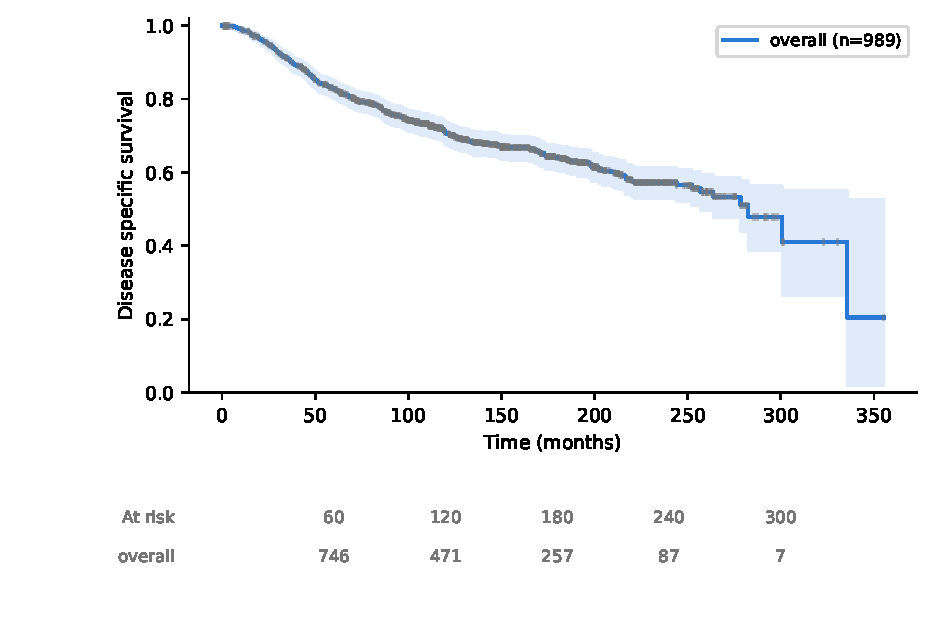
\includegraphics[width=0.82\linewidth]{images/training_disease_specific_overall_km.pdf}
\caption{Kaplan--Meier процена на DSS во тренинг-поделбата ($n=989$), со
95\% pointwise интервали и број на лица под ризик. Малиот број под ризик кон
крајот на следењето ја ограничува прецизноста на доцните процени.}
\label{fig:training-km}
\end{figure}

\subsection{Баесови дијагностики и моделска соодветност}

Сите осум Weibull и sensitivity fit-ови ги исполнија проектните MCMC прагови:
максимален $\widehat R=1.0059$, минимален bulk ESS=1\,714, tail ESS=1\,956 и
нула дивергенции (Табела~\ref{tab:bayes-diagnostics}). Prior-predictive
screening помина кај сите fit-ови, со 1,3--9,3\% симулации надвор од широкиот
опсег. Во posterior predictive проверките, максималното отстапување од
training Kaplan--Meier беше 0,028--0,080; lognormal имаше помали отстапувања,
но локални разлики останаа. Овие проверки се на training-податоците, не
независна потврда. MCMC поминување утврдува семплерска употребливост, не
соодветност на Weibull фамилијата.

\begin{table}[ht]
\centering
\caption{MCMC дијагностики и максимално отстапување во training posterior predictive проверката.}
\label{tab:bayes-diagnostics}
\scriptsize
\begin{tabular}{p{0.35\linewidth}rrrrr}
\hline
Вклопување & max $\widehat R$ & min bulk ESS & min tail ESS & Див. & max $|S-\widehat S_{KM}|$ \\
\hline
DSS Weibull, клинички & 1,0025 & 2\,693 & 2\,419 & 0 & 0,056 \\
DSS Weibull, клинички + PAM50 & 1,0036 & 2\,764 & 2\,539 & 0 & 0,051 \\
OS Weibull, клинички & 1,0059 & 2\,202 & 2\,331 & 0 & 0,075 \\
OS Weibull, клинички + PAM50 & 1,0041 & 2\,313 & 2\,415 & 0 & 0,080 \\
DSS lognormal, клинички & 1,0037 & 1\,780 & 2\,330 & 0 & 0,030 \\
DSS lognormal, клинички + PAM50 & 1,0025 & 3\,049 & 2\,745 & 0 & 0,028 \\
DSS Weibull, поширок prior, клинички & 1,0045 & 2\,204 & 2\,471 & 0 & 0,050 \\
DSS Weibull, поширок prior, клинички + PAM50 & 1,0027 & 1\,714 & 1\,956 & 0 & 0,047 \\
\hline
\end{tabular}
\end{table}

\begin{figure}[ht]
\centering
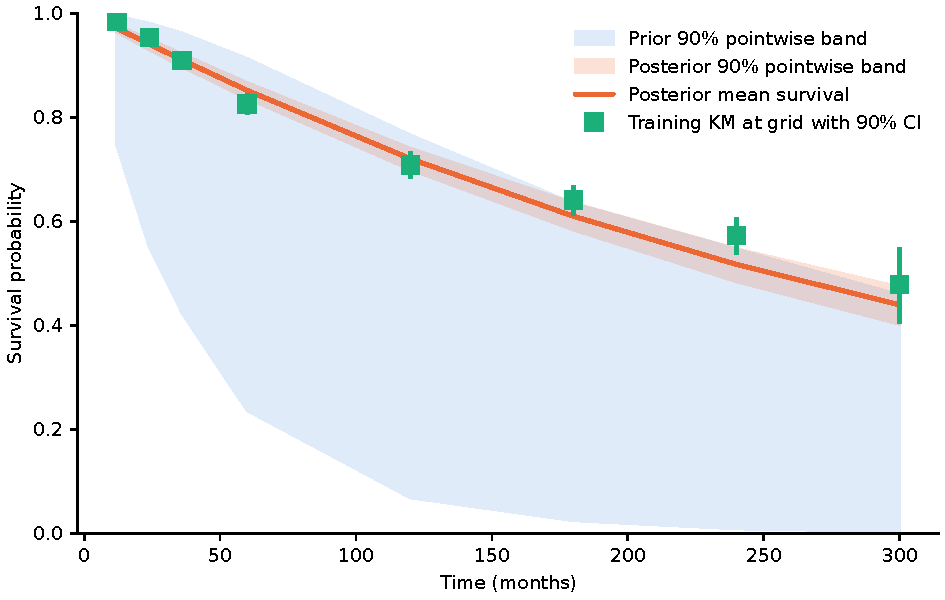
\includegraphics[width=0.48\linewidth]{images/rq4_disease_specific__weibull__clinical_training_ppc.pdf}
\hfill
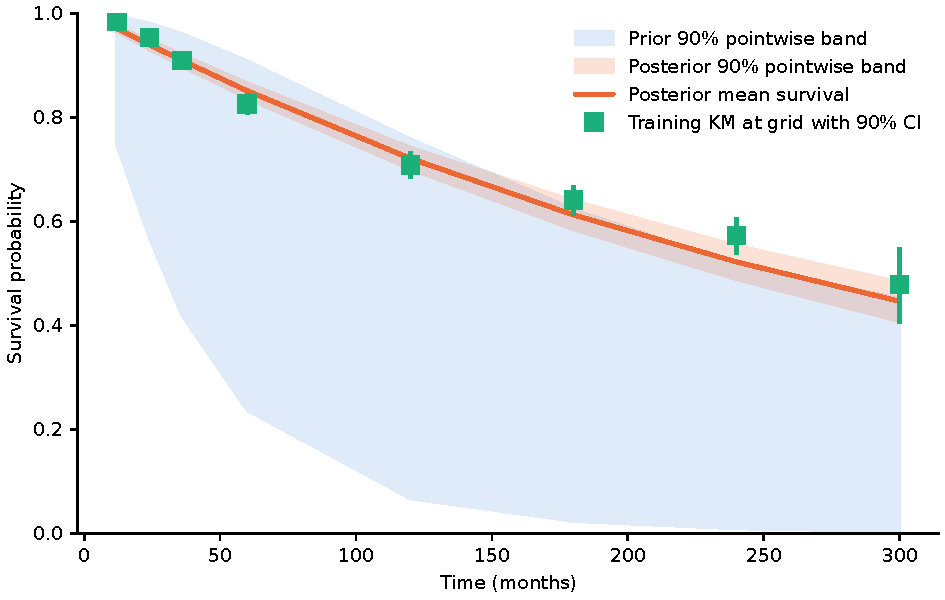
\includegraphics[width=0.48\linewidth]{images/rq4_disease_specific__weibull__clinical_molecular_training_ppc.pdf}
\caption{Training posterior predictive проверка за DSS: клиничкиот Weibull модел (лево) и клиничкиот модел со PAM50 (десно). Прикажани се prior/posterior точковните опсези, средната posterior крива и Kaplan--Meier процените со точковни интервали.}
\label{fig:bayes-training-ppc}
\end{figure}
Prior predictive сликата дополнува процентуален скрининг со временска скала:
за клиничкиот Weibull модел симулираните времиња најчесто се концентрирани на
десетици до неколку стотици месеци, со 1,5\% надвор од прикажаниот опсег.
Ова е визуелна проверка на prior-от условно на тренинг-предикторите, а не
процена на набљудуваното преживување. Таа не кажува дека Weibull фамилијата
соодветно ги опишува податоците; тоа прашање го разгледуваат posterior
predictive проверките и sensitivity споредбата.
\begin{figure}[ht]
\centering
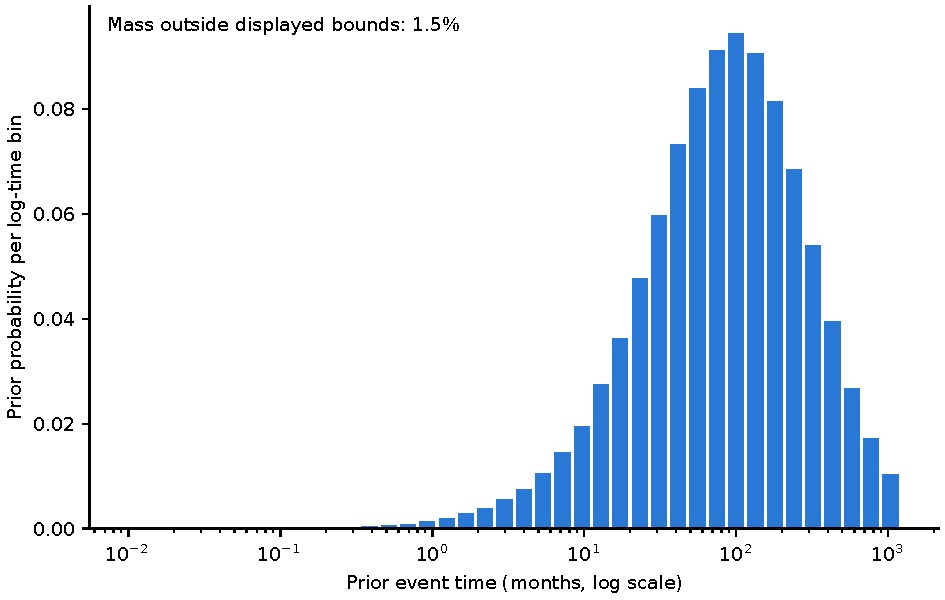
\includegraphics[width=0.82\linewidth]{images/rq4_disease_specific__weibull__clinical_prior_times.pdf}
\caption{Prior predictive распределба на event time-овите за DSS клиничкиот
Weibull модел, симулирани врз тренинг-предикторите. Хоризонталната оска е
логаритамска; прикажаниот опсег е 0,01--1.200 месеци.}
\label{fig:weibull-prior-times}
\end{figure}
Weibull--lognormal разликите во предвидената survival probability зависеа од
хоризонтот. Просечната апсолутна разлика низ training-профилите беше околу
2,1--2,2 процентни поени на 120 месеци и 4,2--4,5 поени на 300 месеци; најголемите
поединечни разлики беа 20,9 и 22,0 поени за клиничкиот и PAM50 моделот.
Поширокиот Weibull prior даде просечни разлики од 0,5--0,6 поени на 120 и
0,9--1,0 поени на 300 месеци; максимумите беа 7,3 и 16,1 поени. Ова се
training-only разлики на кривите, не разлики во event-time месеци. Weibull AFT
со заеднички shape имплицира PH, како и Cox; ниту дијагностиките ниту AFT
параметризацијата го отстрануваат тоа ограничување.

\subsection{Предиктивна точност и придонес на PAM50}

Сите модели се оценети на истите 495 test-пациенти. Интервалите во табелите се
95\% paired percentile-bootstrap интервали од 1\,000 повторувања. Uno C и
динамичката AUC ја мерат дискриминацијата; Brier и IBS ја мерат веројатносната
грешка. IBS се интегрира на train-derived мрежата 28,973--120 месеци.

\begin{table}[ht]
\centering
\caption{DSS дискриминација на тест-подмножество. Ќелиите се процена [95\% bootstrap интервал].}
\label{tab:dss-performance}
\small
\begin{tabular}{llcc}
\hline
Модел & Предиктори & Uno C & Средна динамичка AUC \\
\hline
Cox & Клинички & 0,686 [0,641; 0,730] & 0,745 [0,694; 0,793] \\
Cox & Клинички + PAM50 & 0,696 [0,651; 0,739] & 0,750 [0,696; 0,796] \\
RSF & Клинички & 0,690 [0,645; 0,736] & 0,752 [0,699; 0,799] \\
RSF & Клинички + PAM50 & 0,705 [0,661; 0,748] & 0,766 [0,712; 0,812] \\
Weibull AFT & Клинички & 0,687 [0,642; 0,732] & 0,746 [0,696; 0,792] \\
Weibull AFT & Клинички + PAM50 & 0,705 [0,662; 0,747] & 0,761 [0,709; 0,806] \\
\hline
\end{tabular}
\end{table}
\begin{table}[ht]
\centering
\caption{DSS веројатносна точност на тест-подмножество: пониско е подобро. Ќелиите се процена [95\% bootstrap интервал].}
\label{tab:dss-performance-prob}
\small
\begin{tabular}{llcc}
\hline
Модел & Предиктори & IBS & Brier, 120 месеци \\
\hline
Cox & Клинички & 0,141 [0,129; 0,153] & 0,176 [0,162; 0,193] \\
Cox & Клинички + PAM50 & 0,142 [0,129; 0,154] & 0,178 [0,162; 0,194] \\
RSF & Клинички & 0,140 [0,129; 0,151] & 0,179 [0,166; 0,194] \\
RSF & Клинички + PAM50 & 0,138 [0,128; 0,149] & 0,176 [0,163; 0,191] \\
Weibull AFT & Клинички & 0,143 [0,130; 0,155] & 0,177 [0,163; 0,193] \\
Weibull AFT & Клинички + PAM50 & 0,141 [0,128; 0,154] & 0,175 [0,160; 0,191] \\
\hline
\end{tabular}
\end{table}
Точковните резултати се блиски и интервалите се преклопуваат, па не утврдуваат
единствен најдобар модел. Со PAM50, Cox има Uno C 0,696, RSF и Weibull AFT 0,705;
RSF има најнизок точковен IBS (0,138), а Weibull најнизок Brier на 120 месеци
(0,175). Различниот редослед ја нагласува зависноста од метриката.

\begin{figure}[ht]
\centering
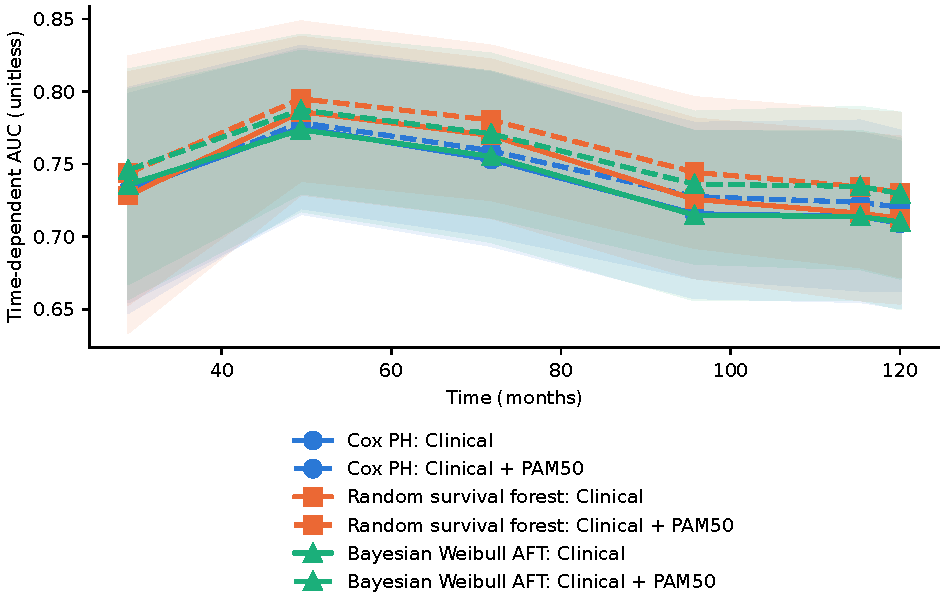
\includegraphics[width=0.49\linewidth]{images/rq1_rq2_rq3_disease_specific_auc.pdf}
\hfill
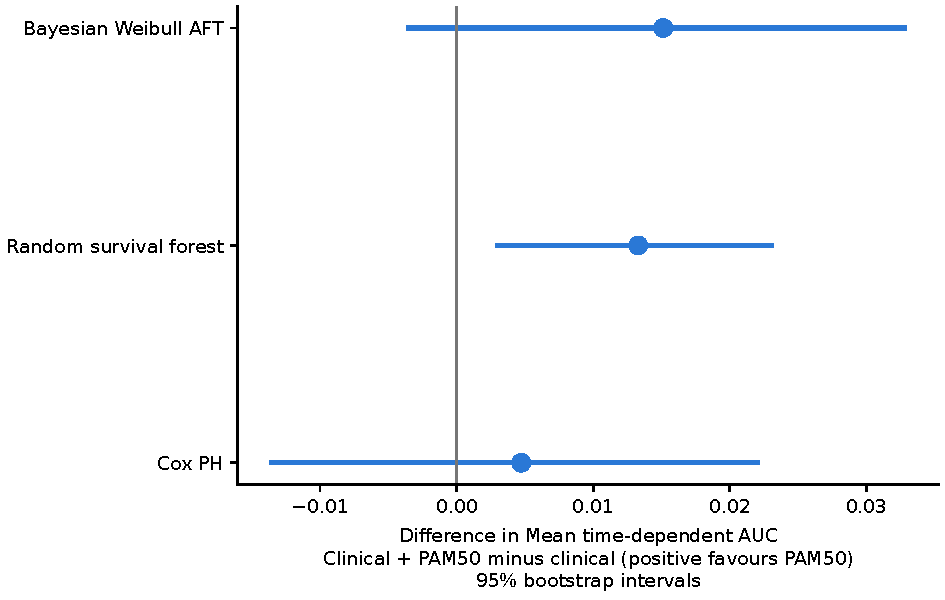
\includegraphics[width=0.49\linewidth]{images/rq1_rq2_rq3_disease_specific_paired_mean_auc.pdf}
\caption{Лево: временски зависна AUC за шесте DSS комбинации модел--feature arm низ заедничката мрежа. Десно: paired разлика во средната динамичка AUC, дефинирана како клинички предиктори плус PAM50 минус клинички предиктори. Прикажаните интервали се 95\% bootstrap интервали.}
\label{fig:dss-auc-comparison}
\end{figure}
Спарените промени од додавањето PAM50 се мали и зависат од моделот
(Табели~\ref{tab:dss-paired-feature-performance} и~\ref{tab:dss-paired-feature-probability}). Кај Cox, сите четири 95\% CI
ја вклучуваат нулата. Кај RSF, интервалите поддржуваат повисок Uno C и AUC и
понизок IBS и Brier. Кај Weibull AFT, само Uno C разликата е јасна; останатите
интервали ја вклучуваат или допираат нулата. Споредбите се експлораторни и без
корекција за повеќекратност.

\begin{table}[ht]
\centering
\caption{Парни DSS разлики во дискриминација меѓу feature arms: клинички + PAM50 минус клинички.}
\label{tab:dss-paired-feature-performance}
\small
\begin{tabular}{lccc}
\hline
Модел & $\Delta$ Uno C & $\Delta$ средна AUC \\
\hline
Cox & 0,010 [-0,005; 0,026] & 0,005 [-0,014; 0,022] \\
RSF & 0,014 [0,003; 0,025] & 0,013 [0,003; 0,023] \\
Weibull AFT & 0,018 [0,003; 0,032] & 0,015 [-0,004; 0,033] \\
\hline
\end{tabular}
\end{table}
\begin{table}[ht]
\centering
\caption{Парни DSS разлики меѓу feature arms за веројатносна точност: клинички + PAM50 минус клинички.}
\label{tab:dss-paired-feature-probability}
\small
\begin{tabular}{lcc}
\hline
Модел & $\Delta$ IBS & $\Delta$ Brier, 120 месеци \\
\hline
Cox & 0,00095 [-0,00203; 0,00486] & 0,00128 [-0,00352; 0,00796] \\
RSF & -0,00180 [-0,00319; -0,00042] & -0,00285 [-0,00545; -0,00007] \\
Weibull AFT & -0,00149 [-0,00306; 0,00004] & -0,00211 [-0,00481; 0,00061] \\
\hline
\end{tabular}
\end{table}
\subsection{OS како анализа на чувствителност}

OS дава различен исход, па неговите абсолютни метрики не се директно споредливи
со DSS. RSF има највисоки точковни Uno C и AUC, но интервалите се преклопуваат;
OS не воспоставува супериорност на моделско семејство и не ја заменува
примарната DSS анализа.

\begin{table}[ht]
\centering
\caption{OS дискриминација на тест-подмножество како анализа на чувствителност. Ќелиите се процена [95\% bootstrap интервал].}
\label{tab:os-performance}
\small
\begin{tabular}{llcc}
\hline
Модел & Предиктори & Uno C & Средна динамичка AUC \\
\hline
Cox & Клинички & 0,649 [0,612; 0,687] & 0,663 [0,615; 0,709] \\
Cox & Клинички + PAM50 & 0,652 [0,616; 0,689] & 0,665 [0,616; 0,711] \\
RSF & Клинички & 0,668 [0,634; 0,700] & 0,722 [0,679; 0,761] \\
RSF & Клинички + PAM50 & 0,678 [0,643; 0,709] & 0,730 [0,686; 0,770] \\
Weibull AFT & Клинички & 0,649 [0,611; 0,686] & 0,664 [0,615; 0,710] \\
Weibull AFT & Клинички + PAM50 & 0,653 [0,616; 0,690] & 0,668 [0,621; 0,713] \\
\hline
\end{tabular}
\end{table}
\begin{table}[ht]
\centering
\caption{OS веројатносна точност на тест-подмножество како анализа на чувствителност. Пониско е подобро; ќелиите се процена [95\% bootstrap интервал].}
\label{tab:os-performance-prob}
\small
\begin{tabular}{llcc}
\hline
Модел & Предиктори & IBS & Brier, 120 месеци \\
\hline
Cox & Клинички & 0,170 [0,155; 0,184] & 0,203 [0,186; 0,219] \\
Cox & Клинички + PAM50 & 0,171 [0,157; 0,185] & 0,204 [0,187; 0,220] \\
RSF & Клинички & 0,162 [0,151; 0,175] & 0,202 [0,190; 0,215] \\
RSF & Клинички + PAM50 & 0,160 [0,149; 0,173] & 0,199 [0,186; 0,211] \\
Weibull AFT & Клинички & 0,170 [0,156; 0,184] & 0,203 [0,187; 0,218] \\
Weibull AFT & Клинички + PAM50 & 0,170 [0,156; 0,184] & 0,203 [0,187; 0,218] \\
\hline
\end{tabular}
\end{table}
\subsection{Conformal покриеност и ефикасност}

При номинални 90\%, DSS score-envelope границите на 300 месеци се приближно
91,5--96,8\%, но медијаните на ширина се 270,8--274,4 месеци: речиси целиот
restricted хоризонт. На 120 месеци медијаните се 90,8--95,1 месеци, со околу
94 месеци за Cox/PAM50. Високата набљудувана покриеност затоа доаѓа со ограничена
прецизност. $\widehat G(120-)=0.6719$ ја поддржува IPCW чувствителноста; на
300 месеци $\widehat G(300-)=0.0148<0.05$, па IPCW е недостапна, а не нула.

\begin{table}[ht]
\centering
\caption{DSS score-envelope резултати при номинално 90\% и хоризонт од 120 месеци. Се прикажуваат набљудуваните coverage граници, IPCW процената со 95\% bootstrap CI и медијаната [Q1; Q3] на ширината. Секој ред има $n_{cal}=495$ и $n_{test}=495$.}
\label{tab:dss-conformal-90-120}
\footnotesize
\setlength{\tabcolsep}{3pt}
\begin{tabular}{p{0.19\textwidth}p{0.17\textwidth}p{0.22\textwidth}p{0.30\textwidth}}
\hline
Модел / feature arm & Coverage граници & IPCW [95\% CI] & Ширина [Q1; Q3] \\
\hline
Cox / clinical & 92,9--95,4\% & 95,0\% [92,9; 96,8] & 94,5 [89,0; 99,0] \\
Cox / clinical + PAM50 & 92,9--95,4\% & 95,0\% [93,0; 96,8] & 94,0 [87,6; 98,8] \\
RSF / clinical & 92,1--95,4\% & 95,1\% [93,1; 96,8] & 90,8 [82,2; 99,0] \\
RSF / clinical + PAM50 & 91,5--95,6\% & 95,3\% [93,3; 97,1] & 91,4 [82,0; 99,0] \\
Weibull / clinical & 93,5--96,2\% & 95,9\% [93,9; 97,4] & 94,5 [85,9; 101,3] \\
Weibull / clinical + PAM50 & 94,5--96,8\% & 96,5\% [94,8; 98,1] & 95,1 [85,3; 102,0] \\
\hline
\end{tabular}
\end{table}

\begin{table}[ht]
\centering
\caption{DSS score-envelope резултати при номинално 90\% и хоризонт од 300 месеци. IPCW нема доволна цензурирачка поддршка до овој хоризонт; медијаната и квартилите на ширината се во месеци. Секој ред има $n_{cal}=495$ и $n_{test}=495$.}
\label{tab:dss-conformal-90-300}
\footnotesize
\setlength{\tabcolsep}{3pt}
\begin{tabular}{p{0.19\textwidth}p{0.17\textwidth}p{0.22\textwidth}p{0.30\textwidth}}
\hline
Модел / feature arm & Coverage граници & IPCW & Ширина [Q1; Q3] \\
\hline
Cox / clinical & 92,9--95,4\% & недостапна & 274,4 [268,4; 279,0] \\
Cox / clinical + PAM50 & 92,5--95,2\% & недостапна & 273,1 [266,8; 278,0] \\
RSF / clinical & 92,1--95,4\% & недостапна & 270,8 [262,2; 279,0] \\
RSF / clinical + PAM50 & 91,5--95,6\% & недостапна & 271,4 [262,0; 279,0] \\
Weibull / clinical & 93,5--96,2\% & недостапна & 274,3 [265,1; 280,8] \\
Weibull / clinical + PAM50 & 94,5--96,8\% & недостапна & 274,3 [264,3; 281,5] \\
\hline
\end{tabular}
\end{table}
\subsubsection{Референтна споредба без предиктори}

Како експлораторна проверка на индивидуализацијата, Kaplan--Meier распределбата
е проценета само на тренинг-поделбата и дава ист почетен интервал за секоја
пациентка. Потоа интервалот е калибриран со истата конзервативна score-envelope
постапка и калибрациската поделба како кај поединечните модели. Kaplan--Meier
проценката за DSS го третира другиот вид смрт како цензурирање и затоа се
толкува како net survival под претпоставка за неинформативно цензурирање; не е
кумулативна инциденца на смрт од рак при competing risks~\cite{kaplan1958,putter2007}.

При главната споредба (90\%, 120 месеци), почетниот KM интервал бил
[24,8; 120] месеци, а по калибрацијата медијаната на ширината била 98,7 месеци.
Набљудуваните coverage граници биле 93,7--95,4\%, а IPCW процената 95,1\%
[93,2; 96,8]. Индивидуалните интервали имале медијани од 90,8 до 95,1 месеци:
за 3,6--7,9 месеци потесни од KM baseline, со спарени bootstrap 95\% интервали
за разликата целосно под нула во сите шест моделско-предикторски комбинации.
Сепак, IPCW разликите во покриеноста не се разликувале јасно од нула; нивните
спарени 95\% интервали ја вклучуваат нулата. Coverage границите не се
набљудување на латентната вистинска покриеност, затоа резултатот е умерен
ефикасносен добивок, а не доказ за поинаква измерена покриеност.

Ниту еден KM или моделски интервал при 90\% и 120 месеци не го покривал целиот
хоризонт; 2,2--8,1\% од моделските интервали биле широки најмалку 90\% од
хоризонтот. И покрај статистички потесните интервали, медијаните од околу
91--95 месеци остануваат широки. Тривијалниот интервал $[0,120]$ има
100\% покриеност по конструкција, но не носи индивидуална прогностичка
информација. Споредбата повторно ја користи веќе отворената тест-поделба и
затоа е пост-хок експлораторна.

% Predictor-free baseline comparison table (kept inline for Overleaf portability).
\begin{table}[htbp]
\centering
\small
\setlength{\tabcolsep}{3pt}
\caption{Референтен модел без предиктори при 90\% номинална покриеност и хоризонт од 120 месеци. Границите се компатибилни со цензурирањето; IPCW бара независно цензурирање и доволна поддршка. Ширината е медијана (интерквартилен распон) во месеци. Пост-хок споредбата на тест-множеството е експлораторна.}
\label{tab:predictor-free-baseline}
\begin{tabular}{@{}lccccc@{}}
\toprule
Метод & Coverage граници & IPCW [95\% CI] & Ширина [медијана (IQR)] & Целосен & Речиси цел \\
\midrule
KM конформал & 93,7\%--95,4\% & 0,951 (0,932; 0,968) & 98,7 (98,7--98,7) & 0,0\% & 0,0\% \\
Тривијален хоризонт & 100,0\%--100,0\% & 1,000 (1,000; 1,000) & 120,0 (120,0--120,0) & 100,0\% & 100,0\% \\
Cox клинички & 92,9\%--95,4\% & 0,950 (0,930; 0,968) & 94,5 (89,0--99,0) & 0,0\% & 2,2\% \\
Cox клин. + PAM50 & 92,9\%--95,4\% & 0,950 (0,930; 0,969) & 94,0 (87,6--98,8) & 0,0\% & 2,8\% \\
Weibull клинички & 93,5\%--96,2\% & 0,959 (0,940; 0,975) & 94,5 (85,9--101,3) & 0,0\% & 8,1\% \\
Weibull клин. + PAM50 & 94,5\%--96,8\% & 0,965 (0,948; 0,979) & 95,1 (85,3--102,0) & 0,0\% & 8,1\% \\
RSF клинички & 92,1\%--95,4\% & 0,951 (0,931; 0,969) & 90,8 (82,2--99,0) & 0,0\% & 4,4\% \\
RSF клин. + PAM50 & 91,5\%--95,6\% & 0,953 (0,933; 0,971) & 91,4 (82,0--99,0) & 0,0\% & 5,3\% \\
\bottomrule
\end{tabular}
\begin{minipage}{0.98\linewidth}\footnotesize
Целосен опсег значи интервал $[0,\tau]$; речиси цел интервал има ширина најмалку 90\% од $\tau$. Тривијалниот интервал има 100\% покриеност по конструкција, но не носи индивидуална информација. Недостапните IPCW процени укажуваат на недоволна цензурирачка поддршка.
\end{minipage}
\end{table}
\begin{figure}[ht]
\centering
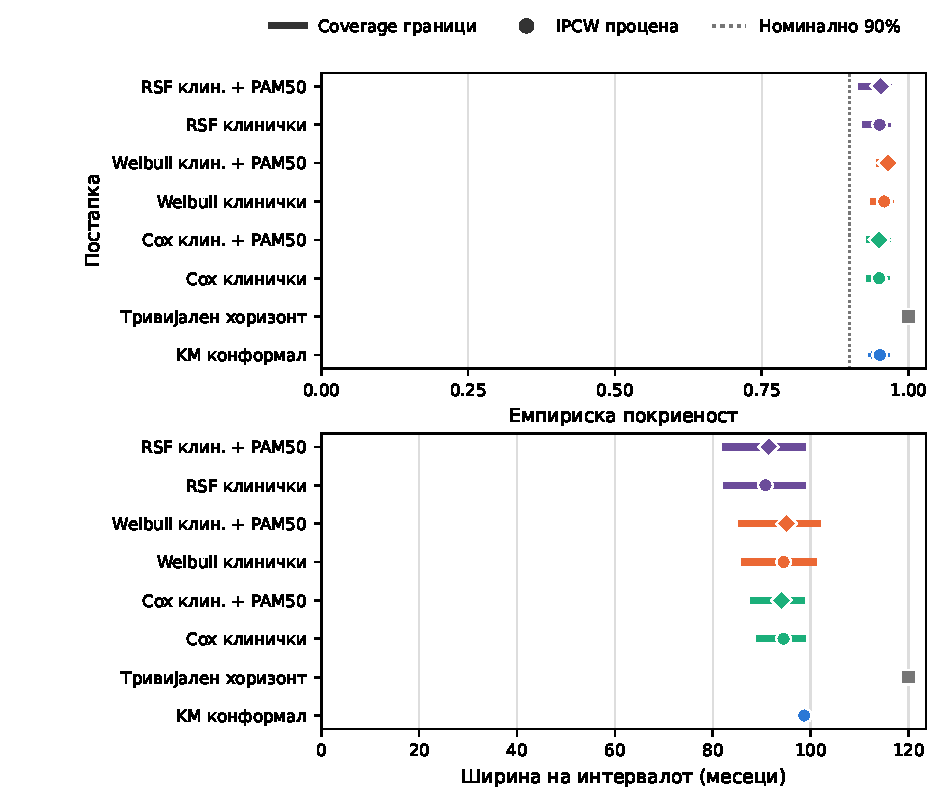
\includegraphics[width=0.88\linewidth]{images/predictor_free_baseline_main.pdf}
\caption{Експлораторна споредба при номинална 90\% покриеност и хоризонт од
120 месеци. Горниот панел ги прикажува набљудуваните граници на покриеност и
IPCW процената со интервал; долниот панел ја прикажува медијаната и
интерквартилниот распон на ширината. Номиналната линија и тривијалниот
интервал се референци, а тест-поделбата е веќе користена во примарната анализа.}
\label{fig:predictor-free-baseline}
\end{figure}

\subsubsection{Баесови предиктивни и конформализирани интервали}

Оваа пост-хок споредба ги користи истите индивидуални posterior predictive
интервали пред и по постојната конформална калибрација. Таа беше дефинирана
откако резултатите од првичниот тест-сет веќе биле разгледани; моделите не се
рефитирани, а калибрациските квантилни вредности не се приспособувани според оваа
тест-споредба. Интервалите се квантилни интервали за
индивидуалното време до настан од posterior predictive распределбата, која
вклучува варијабилност во параметрите и во идното време до настан; тие не се
credible intervals за survival-кривата. При главната споредба (90\%,
120 месеци), калибрацискиот квантил беше нула во двата predictor-сета; затоа
границите на покриеност, IPCW процените и ширините се идентични пред и по
калибрацијата. Медијаните на ширината се 94,5 месеци за клиничкиот сет и
95,1 месеци со PAM50, со набљудливи граници 93,5--96,2\% и 94,5--96,8\%.
Спарените разлики се нула (Табели~\ref{tab:bayesian-conformal-primary-metrics}
и~\ref{tab:bayesian-conformal-primary-differences}).

При номинални 80\% и 120 месеци, калибрацијата ги прошири медијаните за 3,3
месеци кај клиничкиот сет и 1,3 месеци со PAM50. IPCW покриеноста порасна за
1,32 процентни поени кај клиничкиот сет [95\% CI: 0,43; 2,41]; кај клиничкиот
сет со PAM50 промената беше 0,22 поени [95\% CI: 0,00; 0,68], па интервалот
на доверба ја вклучува нулата. Ова покажува дека калибрацијата не додава
секогаш практична ширина или јасно подобрување на покриеноста. Дополнителните
нивоа и хоризонтот од 300 месеци се сумирани во
Табела~\ref{tab:bayesian-conformal-supplement}. При 300 месеци медијаните на
ширината се 250--287 месеци, блиску до целиот хоризонт; IPCW нема доволна
цензурирачка поддршка и не се пријавува. Во сите поставки $n_{test}=495$;
калибрираните интервали користат $n_{cal}=495$ (оригиналните не користат
калибрациски примероци). Во табелите IPCW е дадено како пропорција, а границите
на емпириската покриеност како проценти.

Границите на емпириската покриеност се компатибилни со цензурирањето и не ја
откриваат латентната покриеност за секоја пациентка. IPCW е одделна процена што
претпоставува независно цензурирање и доволна поддршка; bootstrap интервалите
се условни на фиксираните модели, калибрација и тренинг-процена на
цензурирањето. Бидејќи тест-поделбата веќе била разгледана, ова е експлораторна
споредба, не независна валидација или потврда на гаранцијата за покриеност.

% Bayesian predictive vs. conformalized interval tables (inline for Overleaf portability).
\begin{table}[htbp]
\centering
\small
\setlength{\tabcolsep}{4pt}
\caption{Баесови индивидуални предиктивни интервали пред и по конформална калибрација при 90\% номинална покриеност и хоризонт од 120 месеци. Границите се компатибилни со цензурирањето; IPCW претпоставува независно цензурирање. Бројот на тест-пациенти е 495. Ширината е медијана и IQR во месеци.}
\label{tab:bayesian-conformal-primary-metrics}
\begin{tabular}{@{}ll S[table-format=2.1] S[table-format=2.1] l S[table-format=3.1] l@{}}
\toprule
Предиктори & Интервал & {Долна граница, \%} & {Горна граница, \%} & IPCW [95\% CI] & {Медијана, месеци} & IQR \\
\midrule
Клинички & Баесовски предиктивен ($n_{cal}=0$) & 93.5 & 96.2 & 0.959 (0.941; 0.976) & 94.5 & 85.9--101.3 \\
 & конформализиран ($n_{cal}=495$) & 93.5 & 96.2 & 0.959 (0.941; 0.976) & 94.5 & 85.9--101.3 \\
Клинички + PAM50 & Баесовски предиктивен ($n_{cal}=0$) & 94.5 & 96.8 & 0.965 (0.947; 0.980) & 95.1 & 85.3--102.0 \\
 & конформализиран ($n_{cal}=495$) & 94.5 & 96.8 & 0.965 (0.947; 0.980) & 95.1 & 85.3--102.0 \\
\bottomrule
\end{tabular}
\end{table}

\begin{table}[htbp]
\centering
\small
\setlength{\tabcolsep}{3pt}
\caption{Конформализирани минус оригинални Баесови интервали. Прикажани се спарените разлики и 95\% bootstrap интервали за примарната споредба.}
\label{tab:bayesian-conformal-primary-differences}
\begin{tabular}{@{}ll S[table-format=+3.1] S[table-format=+3.1] S[table-format=+3.1]@{}}
\toprule
Предиктори & Мерка & {Разлика} & {95\% CI долна} & {95\% CI горна} \\
\midrule
Клинички & Долна граница покриеност, п.п. & +0.0 & +0.0 & +0.0 \\
Клинички & Горна граница покриеност, п.п. & +0.0 & +0.0 & +0.0 \\
Клинички & IPCW покриеност, п.п. & +0.0 & +0.0 & +0.0 \\
Клинички & Медијана ширина, месеци & +0.0 & +0.0 & +0.0 \\
Клинички + PAM50 & Долна граница покриеност, п.п. & +0.0 & +0.0 & +0.0 \\
Клинички + PAM50 & Горна граница покриеност, п.п. & +0.0 & +0.0 & +0.0 \\
Клинички + PAM50 & IPCW покриеност, п.п. & +0.0 & +0.0 & +0.0 \\
Клинички + PAM50 & Медијана ширина, месеци & +0.0 & +0.0 & +0.0 \\
\bottomrule
\end{tabular}
\end{table}

\begin{table}[htbp]
\centering
\small
\setlength{\tabcolsep}{3pt}
\caption{Дополнителни Баесови и конформализирани резултати за сите регистрирани нивоа и хоризонти. Границите на покриеност и разликите се спарени по тест-пациент; IPCW е прикажан во агрегатниот JSON и е изоставен тука за компактност. При 300 месеци поддршката за IPCW е недоволна.}
\label{tab:bayesian-conformal-supplement}
\begin{tabular}{@{}cc lcc c@{}}
\toprule
Номинална & Хоризонт & Предиктори & Граници: оригинални; конформализирани & Медијана на ширина: оригинална; конформализирана & $\Delta$ ширина [95\% CI] \\
\midrule
95\% & 120 & Клинички & 98.2\%--99.4\%; 98.2\%--99.4\% & 106.5; 106.5 & +0.0 [+0.0; +0.0] \\
95\% & 120 & Клинички + PAM50 & 97.8\%--99.4\%; 97.8\%--99.4\% & 107.0; 107.0 & +0.0 [+0.0; +0.0] \\
95\% & 300 & Клинички & 98.2\%--99.4\%; 98.2\%--99.4\% & 286.5; 286.5 & +0.0 [+0.0; +0.0] \\
95\% & 300 & Клинички + PAM50 & 97.8\%--99.4\%; 97.8\%--99.4\% & 286.6; 286.6 & +0.0 [+0.0; +0.0] \\
90\% & 120 & Клинички & 93.5\%--96.2\%; 93.5\%--96.2\% & 94.5; 94.5 & +0.0 [+0.0; +0.0] \\
90\% & 120 & Клинички + PAM50 & 94.5\%--96.8\%; 94.5\%--96.8\% & 95.1; 95.1 & +0.0 [+0.0; +0.0] \\
90\% & 300 & Клинички & 93.5\%--96.2\%; 93.5\%--96.2\% & 274.3; 274.3 & +0.0 [+0.0; +0.0] \\
90\% & 300 & Клинички + PAM50 & 94.5\%--96.8\%; 94.5\%--96.8\% & 274.3; 274.3 & +0.0 [+0.0; +0.0] \\
80\% & 120 & Клинички & 80.6\%--88.9\%; 82.4\%--90.1\% & 71.1; 74.4 & +3.3 [+3.3; +3.3] \\
80\% & 120 & Клинички + PAM50 & 81.6\%--89.5\%; 82.2\%--89.7\% & 71.9; 73.1 & +1.3 [+1.3; +1.3] \\
80\% & 300 & Клинички & 80.0\%--88.9\%; 82.0\%--90.1\% & 250.1; 253.7 & +3.6 [+3.3; +3.9] \\
80\% & 300 & Клинички + PAM50 & 81.0\%--89.5\%; 81.6\%--89.7\% & 249.9; 251.3 & +1.4 [+1.3; +1.8] \\
\bottomrule
\end{tabular}
\end{table}

Слика~\ref{fig:coverage-width-120} го поставува 120-месечниот резултат во
контекст на неколку различни постапки. Примарниот двостран score-envelope
останува референтен метод; едностраната долна граница и Qin Cox варијантите се
прикажани како експлораторни споредби со различна цел или алгоритам. Тие ги
користат истите веќе анализирани тест-пациенти, па сликата не е независна
валидација и не служи за избор на постапка по резултатот.
\begin{figure}[ht]
\centering
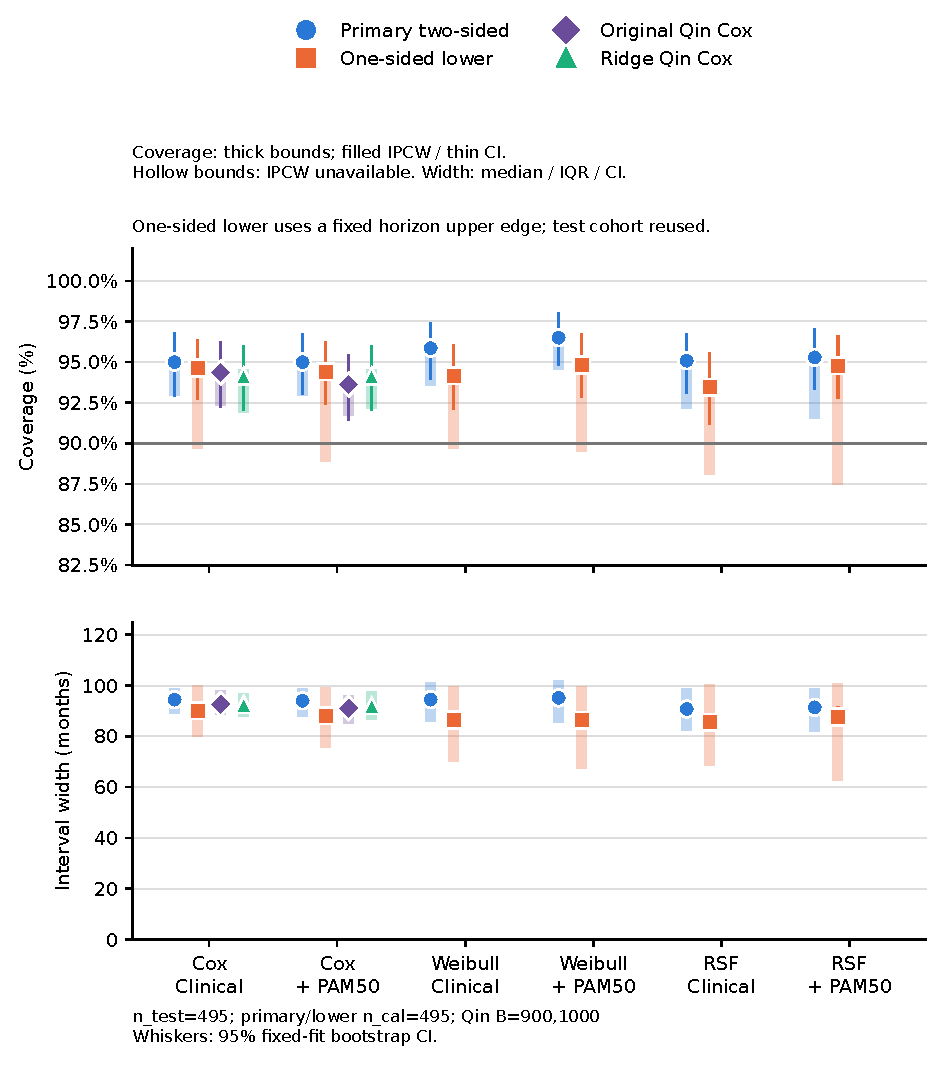
\includegraphics[width=0.82\linewidth]{images/reliability_coverage_width__disease_specific__horizon120__nominal0.90.pdf}
\caption{DSS покриеност и ширина на 120 месеци при номинално 90\%. Дебели
ознаки ги прикажуваат набљудуваните граници на покриеност, а долниот панел
медијана, интерквартилен распон и 95\% fixed-fit bootstrap интервал за ширина.
IPCW е прикажана кога поддршката ја дозволува. Примарниот score-envelope,
едностраната и Qin варијантите имаат различни цели и процени; последните две
се пост-хок и се прикажани само како експлораторни чувствителности.}
\label{fig:coverage-width-120}
\end{figure}
\begin{figure}[ht]
\centering

\centering
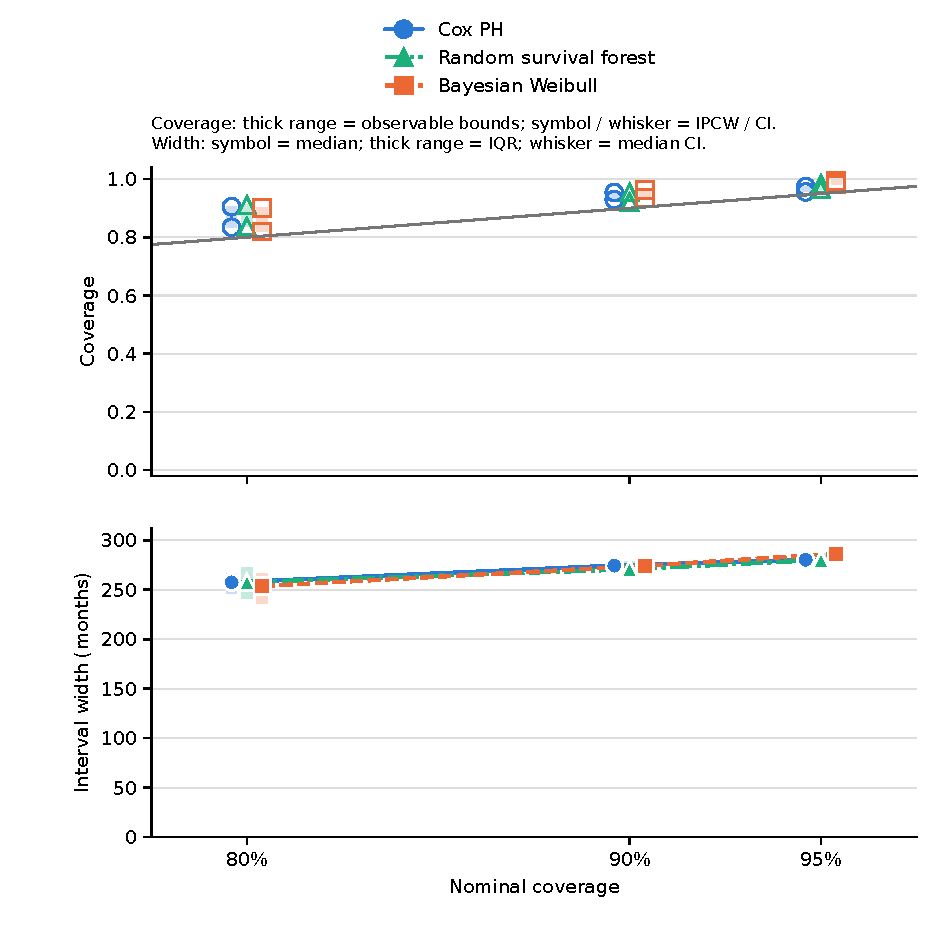
\includegraphics[width=0.88\linewidth]{images/rq5_coverage_vs_nominal__disease_specific__clinical__conservative__horizon300.pdf}
\caption{DSS conformal покриеност и ширина за ограниченото време
$\min(T,300)$ со score-envelope методот и клинички предиктори. Хоризонталната
линија ја означува номиналната покриеност; дебелите вертикални распони се
набљудуваните граници, а отворените ознаки ги покажуваат границите кога IPCW е
недостапен. Долниот панел прикажува медијана и интерквартилен распон на
ширината; интервалите се условни на фиксните модели и калибрација.}
\label{fig:dss-conformal-300-clinical}
\end{figure}

\clearpage
\begin{figure}[ht]
\centering
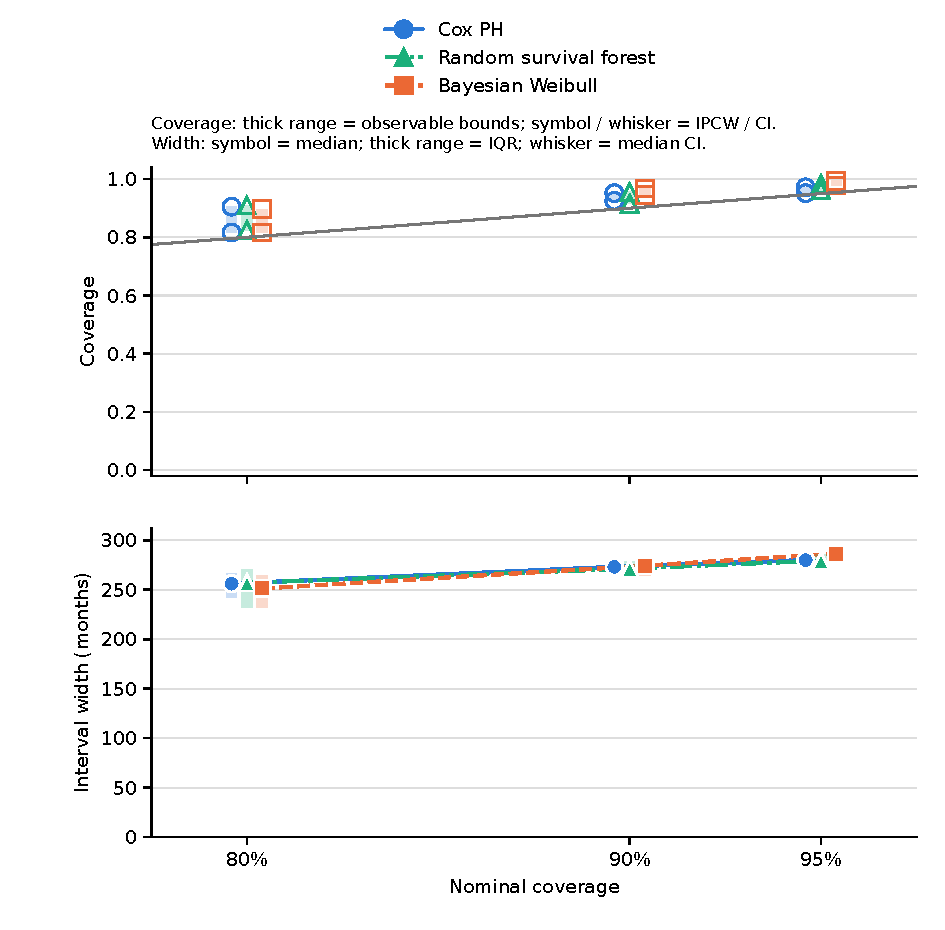
\includegraphics[width=0.88\linewidth]{images/rq5_coverage_vs_nominal__disease_specific__clinical_molecular__conservative__horizon300.pdf}
\caption{DSS conformal покриеност и ширина за ограниченото време
$\min(T,300)$ со score-envelope методот и клинички предиктори плус PAM50.
Хоризонталната линија ја означува номиналната покриеност; дебелите вертикални
распони се набљудуваните граници, а отворените ознаки ги покажуваат границите
кога IPCW е недостапен. Долниот панел прикажува медијана и интерквартилен распон
на ширината; интервалите се условни на фиксните модели и калибрација.}
\label{fig:dss-conformal-300-molecular}
\end{figure}

Набљудливите граници се идентификациски граници на реализираната покриеност,
не CI за латентната вистинска покриеност; bootstrap CI за секоја граница ја
опишува примерочната варијација на индикаторот. IPCW е одделна процена под
посилна независност на цензурирањето. Парните промени во двете coverage граници
по додавање PAM50 ги вклучуваат нулата кај сите модели. Единствената разлика во
ширината чиј CI ја исклучува нулата е Cox, со намалување од околу 1,27 месеци;
тоа е мало во однос на 271--274 месеци ширина на 300-месечниот хоризонт.

\begin{table}[ht]
\centering
\caption{Парни разлики во DSS conformal покриеност и медијана на ширина:
клинички + PAM50 минус клинички; процена [95\% bootstrap интервал].}
\label{tab:dss-pam50-coverage-delta}
\scriptsize
\begin{tabular}{lccc}
\hline
Модел & $\Delta$ долна граница & $\Delta$ горна граница & $\Delta$ медијана на ширина (месеци) \\
\hline
Cox & -0,004 [-0,012; 0,004] & -0,002 [-0,008; 0,004] & -1,27 [-1,47; -0,37] \\
RSF & -0,006 [-0,020; 0,006] & 0,002 [-0,006; 0,010] & 0,63 [0,00; 1,13] \\
Weibull AFT & 0,010 [-0,002; 0,022] & 0,006 [-0,004; 0,016] & 0,02 [-0,67; 1,38] \\
\hline
\end{tabular}
\end{table}
\subsubsection{Подгрупи}

Подгрупните опсези низ шесте модел-feature комбинации се описни, не гаранции за
условна coverage. Кај Basal ($n=59$), точковните горни граници се 84,7--94,9\%
и интервалите се широки; за ER-негативната група ($n=130$) се 91,5--95,4\%.
Интервалите и ширините остануваат големи, а PAM50 \texttt{unknown} ($n=3$) е
потиснат под прагот. Нема корекција за повеќекратни подгрупни споредби.

\begin{table}[ht]
\centering
\caption{DSS subgroup summary at nominal 90\% and 300 months using score-envelope intervals. For coverage, the point-estimate ranges and 95\% bootstrap CI envelopes are shown; width gives the median range and its CI envelope across six model--feature combinations.}
\label{tab:dss-subgroup-summary}
\small
\begin{tabular}{p{0.17\textwidth}p{0.77\textwidth}}
\hline
Подгрупа & Сумарни процени [опсег на 95\% CI] \\
\hline
PAM50: Basal & $n=59$; долна coverage граница 83,1--93,2\% [74,6--98,3\%]; горна 84,7--94,9\% [76,3--100,0\%]; медијана на ширина 279,9--284,4 [278,0--285,2] месеци. \\
PAM50: Her2 & $n=54$; долна coverage граница 88,9--90,7\% [79,6--98,1\%]; горна 90,7--92,6\% [83,3--98,1\%]; медијана на ширина 278,1--282,3 [274,9--284,2] месеци. \\
PAM50: LumA & $n=172$; долна coverage граница 90,7--95,9\% [86,6--98,8\%]; горна 97,1--98,8\% [94,8--100,0\%]; медијана на ширина 257,0--271,4 [253,3--272,2] месеци. \\
PAM50: LumB & $n=108$; долна coverage граница 96,3--98,1\% [92,6--100,0\%]; горна 97,2--99,1\% [94,4--100,0\%]; медијана на ширина 270,3--277,6 [269,1--278,4] месеци. \\
PAM50: Normal & $n=36$; долна coverage граница 80,6--97,2\% [66,7--100,0\%]; горна 94,4--100,0\% [86,1--100,0\%]; медијана на ширина 268,5--275,4 [265,7--278,5] месеци. \\
PAM50: claudin-low & $n=63$; долна coverage граница 90,5--92,1\% [84,1--98,4\%]; горна 93,7--95,2\% [87,3--100,0\%]; медијана на ширина 271,8--277,1 [269,0--279,6] месеци. \\
ER негативен & $n=130$; долна coverage граница 89,2--93,1\% [83,8--96,9\%]; горна 91,5--95,4\% [86,9--98,5\%]; медијана на ширина 279,6--282,6 [278,0--283,9] месеци. \\
ER позитивен & $n=365$; долна coverage граница 91,2--95,1\% [88,2--97,0\%]; горна 95,9--97,3\% [94,0--98,6\%]; медијана на ширина 266,1--272,7 [264,8--273,3] месеци. \\
\hline
\end{tabular}
\end{table}
\subsubsection{Пост-хок методски чувствителности}

Qin Cox bootstrap, ridge Qin и едностраните граници се пост-хок и одговараат на
различни цели или алгоритми. На 120 месеци нивните ширини се малку помали од
примарните, но не се избираат по ширина: Qin има Cox working model и приближна
валидност, а првичниот DSS/PAM50 refit успеа во 900/1\,000 повторувања, точно на
минималниот gate. Ridge варијантата успеа во 1\,000/1\,000, што ја подобрува
нумеричката стабилност, не цензурирачката поддршка. На 300 месеци IPCW останува
недостапна, а интервалите се широки. Сите споредби повторно го користат веќе
отворениот test set.

\begin{table}[ht]
\centering
\caption{DSS method sensitivity at 120 months and nominal 90\%. Observable coverage bounds, IPCW estimate with 95\% bootstrap CI, and median width with its 95\% CI are separate. Qin $B$ counts successful refits out of 1,000; each row uses $n_{cal}=n_{test}=495$.}
\label{tab:dss-method-sensitivities}
\footnotesize
\setlength{\tabcolsep}{3pt}
\begin{tabular}{p{0.30\textwidth}p{0.16\textwidth}p{0.20\textwidth}p{0.24\textwidth}}
\hline
Метод и цел & Coverage граници & IPCW [95\% CI] & Ширина [95\% CI], месеци \\
\hline
Score-envelope, примарен двостран интервал & 92,9--95,4\% & 95,0\% [93,0; 96,8] & 94,0 [93,0; 94,5] \\
IPCW score, двостран интервал & 92,1--94,5\% & 94,1\% [92,0; 96,0] & 92,0 [91,0; 92,5] \\
Signed score-envelope, пост-хок долна граница $[L,\tau]$ & 88,9--94,7\% & 94,4\% [92,4; 96,3] & 88,1 [86,7; 89,6] \\
Qin Cox bootstrap, пост-хок двостран ($B=900/1.000$) & 91,7--94,1\% & 93,6\% [91,4; 95,5] & 91,1 [90,8; 92,1] \\
Ridge Qin, пост-хок двостран, казна 1,0 ($B=1.000/1.000$) & 92,1--94,5\% & 94,1\% [92,0; 96,0] & 92,0 [91,1; 92,5] \\
\hline
\end{tabular}
\end{table}

\begin{table}[ht]
\centering
\caption{DSS method sensitivity at 300 months and nominal 90\%. IPCW coverage is unavailable because censoring support is insufficient; widths are in months. Qin $B$ counts successful refits out of 1,000; each row uses $n_{cal}=n_{test}=495$.}
\label{tab:dss-method-sensitivities-300}
\footnotesize
\setlength{\tabcolsep}{3pt}
\begin{tabular}{p{0.30\textwidth}p{0.16\textwidth}p{0.20\textwidth}p{0.24\textwidth}}
\hline
Метод и цел & Coverage граници & IPCW & Ширина [95\% CI], месеци \\
\hline
Score-envelope, примарен двостран интервал & 92,5--95,2\% & недостапна & 273,1 [272,7; 274,0] \\
IPCW score, двострана целосна поддршка & 100,0--100,0\% & недостапна & 300,0 [300,0; 300,0] \\
Signed score-envelope, пост-хок долна граница $[L,\tau]$ & 88,9--94,7\% & недостапна & 268,1 [266,7; 269,6] \\
Qin Cox bootstrap, пост-хок двостран ($B=900/1.000$) & 89,3--94,1\% & недостапна & 270,3 [269,6; 271,0] \\
Ridge Qin, пост-хок двостран, казна 1,0 ($B=1.000/1.000$) & 89,7--94,3\% & недостапна & 270,9 [269,9; 271,5] \\
\hline
\end{tabular}
\end{table}
\subsubsection{Case-mix стрес-тест}

Пост-хок стрес-тестот ги препондерира истите 495 test-пациенти со фиксирани
модели и калибрација. За Cox/PAM50 при 90\% и 120 месеци, Basal-enrichment
сценариото имаше набљудливи граници 91,9--94,2\%, медијана на ширина 94,5 месеци
и ESS 456,7; базното сценарио беше 92,9--95,4\%, 94,0 месеци и ESS 495.
Сценаријата со помлада/постара возраст беа слични, со ESS околу 404--409.
Ова покажува чувствителност на конкретните тежини, не надворешна валидација,
нова кохорта или гаранција под distribution shift.

\clearpage
\subsection{Кратки одговори на истражувачките прашања}

\begin{enumerate}
\item Клиничките модели даваат умерена, слична DSS дискриминација; нивните CI се преклопуваат (Табели~\ref{tab:dss-performance} и~\ref{tab:dss-performance-prob}).
\item PAM50 дава скромни, модел-зависни добивки: најдоследни кај RSF, ограничени кај Cox и јасни главно за Uno C кај Weibull; споредбите се експлораторни (Табели~\ref{tab:dss-paired-feature-performance} и~\ref{tab:dss-paired-feature-probability}).
\item Метриките не рангираат исто: RSF има најнизок IBS, Weibull најнизок 120-месечен Brier; нема стабилен победник.
\item MCMC дијагностиките поминуваат, но Weibull adequacy е ограничена од PPC, семејната чувствителност и PH претпоставката.
\item Score-envelope границите се над номиналните во оваа поделба, но интервалите се широки; на 300 месеци IPCW нема поддршка (Табели~\ref{tab:dss-conformal-90-120} и~\ref{tab:dss-conformal-90-300}).
\item Подобра дискриминација не значи поинформативна uncertainty. Во пост-хок Баесовата споредба, калибрацијата не ги измени интервалите при 90\% и 120 месеци; валидноста и ефикасноста се оценуваат одделно.
\end{enumerate}

\section{Дискусија}

\subsection{Главни наоди и PAM50}

Трите моделски семејства покажаа блиска, умерена дискриминација за примарниот
DSS исход, без стабилен победник низ метриките. Додавањето PAM50 даде мали
спарени добивки: кај RSF разликите беа најдоследни, кај Weibull најјасни за
Uno C, а кај Cox интервалите на доверба ги опфаќаа нултите разлики. Ова е
согласност со ограничен прогностички придонес во оваа кохорта, не доказ дека
PAM50 секогаш ја подобрува прогнозата. Резултатот се однесува само на додадена
категоријална PAM50 ознака, не на целосни геномски или експресиски профили.

Овој образец треба да се споредува внимателно со претходната METABRIC работа,
бидејќи таа користела различни исходи, предиктори и протоколи
~\cite{neapolitan2015}. Пошироките benchmark студии исто покажуваат дека
заклучокот за модел зависи од метриката и поделбата~\cite{wissel2025}. Во оваа
работа, point-estimate подобрување не е само по себе убедлив доказ: важни се
спарените CI, преклопувањето на моделските интервали и отсуството на корекција
за повеќекратни споредби.

\subsection{Точност, Bayesian неизвесност и моделски претпоставки}

Uno C и временската AUC го оценуваат рангирањето; Brier и IBS ја оценуваат
веројатносната грешка. Тие може да дадат различен редослед, па не оправдуваат
единечно рангирање. Bayesian credible bands ја опишуваат неизвесноста за
условната survival функција, а индивидуалниот posterior predictive интервал
додава варијабилност на времето до настан. Ниту едниот е conformal coverage
резултат.

MCMC дијагностиките покажуваат дека posterior-от бил семплиран според зададените
критериуми, но training PPC отстапувањата и Weibull/lognormal разликите го
ограничуваат заклучокот за соодветност. Просечните апсолутни разлики на кривите
се околу 2 процентни поени на 120 месеци и 4--5 на 300 месеци, со поголеми
максимални индивидуални разлики. Алтернативната фамилија затоа има видливо
влијание, особено во подоцнежниот опсег; чувствителноста не е избрана според
test. Дополнително, и Cox PH и заеднички-shape Weibull AFT подразбираат
пропорционални хазарди. AFT формата не го решава автоматски PH отстапувањето.
Доцните Weibull предвидувања се параметарска екстраполација со долги опашки,
не клинички прогнози.

\subsection{Conformal validity и ефикасност}

Номиналната покриеност е целта на процедурата, не резултат измерен во примерокот.
Поради цензурирањето, вистинската тест-покриеност не е позната за секој пациент;
score-envelope резултатите затоа прикажуваат набљудливи долна и горна граница.
Bootstrap CI се однесуваат на примерочната неизвесност на тие граници, не на
латентната покриеност. IPCW е трета, одделна процена која бара маргинално
независно цензурирање и доволна поддршка. Овие три величини не се заменливи.

Примарната конзервативна калибрација го користи најлошиот score компатибилен со
интервалниот исход и event-стратификувана разменливост; тоа поддржува маргинален
резултат за ограниченото време под наведените претпоставки. Не гарантира
условна покриеност за секој профил, подгрупа или друга кохорта. Candès, Lei и
Ren анализираат специфична поставка за цензурирање и долни граници, додека
Qin et al. развиваат bootstrap Cox-пристап со повторни fit-ови
~\cite{candes2023,qin2025}. Нашата score-envelope постапка е одделна, поконзервативна
адаптација; Qin споредбите, едностраните граници и ridge се пост-хок и не смеат
да се претстават како потврдна селекција на метод. Теоретската рамка за split
conformal е дадена од Angelopoulos и Bates~\cite{angelopoulos2023}.

Покриеноста сама по себе не ја мери практичната информативност. На 120 месеци
медијаната на ширина е околу 94 месеци; на примарните 300 месеци е околу
271--274 месеци од можни 300. Тоа значи дека интервалите се блиску до целиот
restricted хоризонт и имаат ограничена вредност за прецизна индивидуална
прогноза, дури и кога набљудливите долни граници се над номиналното ниво.
Ова е суштинската разлика меѓу validity и efficiency: формално оправдана
покриеност не гарантира тесен, корисен интервал. Кај 300 месеци цензурирачката
поддршка е недоволна за IPCW, па не се пријавува процена за тој опсег.

Подгрупните процени се пошироко неизвесни, особено кај помалите групи како
Basal. Маргинална coverage не повлекува coverage условно на PAM50 или ER;
резултатите се описни и без multiplicity correction. Оваа разлика важна е и
за интерпретација на можни fairness или clinical utility тврдења, кои оваа
анализа не утврдува.

\subsection{DSS, применливост и ограничувања}

Кај DSS, цензурирањето на смрт од друга причина го прави исходот cause-specific
или net survival под претпоставки; не ја проценува реалната кумулативна
инциденца на смрт од рак во присуство на конкурентните смртни случаи
~\cite{putter2007,austin2016}. OS е соодветната поширока чувствителност, но не
го менува примарниот estimand. Оваа разлика го ограничува клиничкото толкување
на DSS-временските процени.

Резултатите потекнуваат од една историска METABRIC кохорта и една замрзната
поделба. Возрасните и Basal case-mix тежини ја менуваат само евалуацијата на
истите тест-пациенти со фиксирани модели и calibration; тоа е локален стрес-тест,
не независна надворешна валидација. TCGA-BRCA не ги има сите оригинални
предиктори и споредливиот DSS исход за валидирање на истите fit-ови, па не е
прикажан како валидациски резултат. Потребна е независна кохорта со соодветни
предиктори, исход и follow-up за такво тврдење.

Ограничувањата вклучуваат зависност од цензурирачките претпоставки, слабата
поддршка до 300 месеци, можните PH отстапувања, Weibull tail спецификацијата,
единечната поделба и условните fixed-fit bootstrap CI. Пост-хок Qin и shift
анализите се експлораторни. Чистото повторување ги усогласи примарните
агрегати со зачуваните резултати, но алтернативните prior MCMC сумирања имаа
мала документирана Monte Carlo варијација; точната граница е наведена во
репродуцибилниот пакет.

\subsection{Практични импликации}

Практичниот придонес е методолошки: споредбата на survival модели треба да ги
раздели дискриминацијата, веројатносната точност, Bayesian predictive
неизвесноста и conformal coverage, а интервалите да ги пријавува со ширина и
цензурирачка поддршка. Во оваа кохорта, ниту повисок point estimate ниту висока
набљудувана долна граница сами по себе утврдуваат клиничка корисност. Анализата
е истражувачка, не е клинички систем и не поддржува индивидуални одлуки за
лекување.

\section{Заклучок и идна работа}

Во оваа METABRIC споредба, клиничките Cox PH, Weibull AFT и RSF модели имаа
слична умерена DSS дискриминација; додавањето PAM50 даде скромни, модел-зависни
промени, без универзален победник. Баесовите дијагностики беа прифатливи, но
PPC, разликите Weibull--lognormal и PH претпоставката ја ограничуваат
моделската интерпретација. Примарните conformal интервали покажаа набљудувани
граници над номиналното ниво во оваа поделба, но медијаната на ширина беше околу
94 месеци на хоризонт од 120 и 271--274 месеци на 300. Пост-хок споредбата
покажа дека при 90\% и 120 месеци калибрацискиот квантил бил нула, па Баесовите
интервали не се измениле; при 80\% тие се прошириле умерено, со нееднакво јасни
промени во проценетата покриеност. Затоа валидноста не значи и доволна
ефикасност или практична информативност. DSS се толкува како net
survival под цензурирачки претпоставки, OS останува чувствителност, а надворешна
валидација не е утврдена.

Приоритетна идна работа е: (1) независна кохорта со споредливи оригинални
предиктори, endpoint и follow-up; (2) временски калибрирана евалуација со
доволна поддршка во доцните хоризонти; (3) competing-risk анализа на кумулативна
инциденца ако истражувачкото прашање го бара тој estimand; (4) проверка на
missingness стратегиите и стабилност низ нови поделби; и (5) дополнителна
проверка или проширување на моделските фамилии кога PH и Weibull претпоставките
се несоодветни. TCGA може да се разгледа само по audit дека ги содржи сите
потребни предиктори и споредлив исход; намалено-feature refit не ја валидира
оригиналната спецификација.

\section{Конфигурациски вредности}

Овој додаток ги собира параметрите потребни за повторување на главниот
експеримент. Табела~\ref{tab:appendix-config} ги сумира вредностите од
\texttt{config/default.yaml}; деталите за нивната методолошка улога се дадени
во поглавјата за дизајнот, моделите и евалуацијата.

\begin{table}[ht]
\centering
\caption{Клучни конфигурациски вредности за примарната анализа.}
\label{tab:appendix-config}
\small
\begin{tabular}{p{0.24\linewidth}p{0.68\linewidth}}
\hline
Поставка & Вредност \\
\hline
Семе & 8927 \\
Поделба & 50\% тренинг, 25\% калибрација, 25\% тест; стратификација според настан \\
Предикторски множества & Клинички: возраст, големина и градус на тумор, позитивни лимфни јазли, ER, PR, HER2; проширено: клинички предиктори плус PAM50 \\
Исходи & Примарен DSS; OS како анализа на чувствителност \\
Conformal хоризонти и нивоа & 300 месеци примарно, 120 месеци секундарно; $\alpha\in\{0{,}20,0{,}10,0{,}05\}$, односно номинални 80\%, 90\%, 95\% \\
Conformal методи & Конзервативен score-envelope; IPCW како анализа на чувствителност \\
Bootstrap & 1\,000 повторувања; 95\% интервали; евалуациска временска мрежа од 10-ти до 90-ти перцентил на следењето \\
Cox PH & Нерегуларизиран модел ($\alpha=0$), Breslow врски \\
Баесов семплер & 4 синџири; 1\,000 warmup и 1\,000 задржани извлекувања по синџир; target acceptance 0,95 \\
Баесова капија & Максимум $\widehat{R}=1{,}01$; минимум bulk и tail ESS од 400; нула дивергенции \\
Weibull prior & Пресек $\mathcal{N}(\log 120,0{,}5^2)$; коефициенти $\mathcal{N}(0,0{,}35^2)$; log-shape $\mathcal{N}(\log 1{,}5,0{,}35^2)$ \\
Prior чувствителност & Weibull: SD 0,75 за пресекот и 0,70 за коефициентите; lognormal: скала HalfNormal(0,75) \\
Random Survival Forest & 500 дрва; минимален лист 15; минимален split 10; $\sqrt{p}$ предиктори по split \\
\hline
\end{tabular}
\end{table}

Додатокот ги наведува конфигурациските вредности за примарната анализа; резултатите и дијагностиките се прикажани во соодветните поглавја.

\section{Репродуцибилност и пристап до податоците}

Примарната анализа е повторена од чиста ревизија на кодот со документирани
конфигурации, SHA-256 манифести и SLURM логови. Кохортата и поделбата од
989/495/495 се реконструирани, а клучните примарни агрегати за кохортата,
метриките, спарените feature-set разлики, conformal резултатите и одговорите на
истражувачките прашања се совпаѓаат со зачуваните резултати. Посебните Qin и
reliability агрегати исто така се совпаднале. Кај алтернативните prior Weibull
MCMC fit-ови имало мала Monte Carlo варијација меѓу повторувањата; дијагностичките
прагови биле исполнети, а главниот заклучок за чувствителноста останал ист.
Оттука, тврдењето е репродукција на клучните агрегатни резултати, а не
бит-по-бит идентичност на сите posterior извлекувања.

Деталните конфигурации, верзии, логови, манифести, checksum проверки и
резултати од споредбата се достапни во
\href{https://github.com/TheeOliver/brca-survival-uncertainty/tree/main/docs/reproducibility/2026-10-30}{пакетот за репродуцибилност}.
За повторување од чист checkout, по поставувањето и проверката на клиничката
METABRIC снимка, документирани се следните SLURM повици:
\begin{verbatim}
sbatch scripts/slurm/run_pipeline.sh config/default.yaml
sbatch scripts/slurm/run_stage.sh 05 config/default.yaml \
  --qin-exploratory
sbatch scripts/slurm/run_stage.sh 05 config/default.yaml \
  --reliability-exploratory
\end{verbatim}
Проширувањата со Qin и reliability се пост-хок и се чуваат одделно од
примарниот pipeline. Анализите на модели, калибрација, тест и bootstrap се
извршени на SLURM compute-јазли, а не на login host. Клиничките табели и нивните
четири SHA-256 проверки се достапни во
\href{https://github.com/TheeOliver/brca-survival-uncertainty/tree/main/data/raw/cbioportal_brca_metabric}{јавниот репозиториум};
целосните контролирани експресиски матрици не се користат или прераспределуваат.
Оваа документација овозможува пристап до точната клиничка снимка употребена во
анализата, но не ја претвора анализата во независна надворешна валидација.

\begin{thebibliography}{99}

\bibitem{curtis2012}
C. Curtis et al., ``The genomic and transcriptomic architecture of 2,000 breast
tumours reveals novel subgroups,'' \textit{Nature}, vol. 486, no. 7403,
pp. 346--352, 2012. doi: \href{https://doi.org/10.1038/nature10983}{10.1038/nature10983}.

\bibitem{neapolitan2015}
R. E. Neapolitan and X. Jiang, ``Study of integrated heterogeneous data reveals
prognostic power of gene expression for breast cancer survival,''
\textit{PLOS ONE}, vol. 10, no. 2, e0117658, 2015.
doi: \href{https://doi.org/10.1371/journal.pone.0117658}{10.1371/journal.pone.0117658}.

\bibitem{angelopoulos2023}
A. N. Angelopoulos and S. Bates, ``A gentle introduction to conformal prediction
and distribution-free uncertainty quantification,'' arXiv:2107.07511, 2023.
URL: \href{https://arxiv.org/abs/2107.07511}{arXiv preprint}.

\bibitem{candes2023}
E. Candès, L. Lei, and Z. Ren, ``Conformalized survival analysis,''
\textit{Journal of the Royal Statistical Society: Series B (Statistical Methodology)},
vol. 85, no. 1, pp. 24--45, 2023.
doi: \href{https://doi.org/10.1093/jrsssb/qkac004}{10.1093/jrsssb/qkac004}.

\bibitem{wissel2025}
D. Wissel et al., ``SurvBoard: standardized benchmarking for multi-omics cancer
survival models,'' \textit{Briefings in Bioinformatics}, vol. 26, no. 5,
bbaf521, 2025.
doi: \href{https://doi.org/10.1093/bib/bbaf521}{10.1093/bib/bbaf521}.

\bibitem{gui2024}
Y. Gui, R. Hore, Z. Ren, and R. F. Barber, ``Conformalized survival analysis
with adaptive cut-offs,'' \textit{Biometrika}, vol. 111, no. 2,
pp. 459--477, 2024.
doi: \href{https://doi.org/10.1093/biomet/asad076}{10.1093/biomet/asad076}.

\bibitem{cerami2012}
E. Cerami et al., ``The cBio cancer genomics portal: An open platform for
exploring multidimensional cancer genomics data,'' \textit{Cancer Discovery},
vol. 2, no. 5, pp. 401--404, 2012.
doi: \href{https://doi.org/10.1158/2159-8290.CD-12-0095}{10.1158/2159-8290.CD-12-0095}.

\bibitem{gao2013}
J. Gao et al., ``Integrative analysis of complex cancer genomics and clinical
profiles using the cBioPortal,'' \textit{Science Signaling}, vol. 6, no. 269,
pl1, 2013.
doi: \href{https://doi.org/10.1126/scisignal.2004088}{10.1126/scisignal.2004088}.

\bibitem{pereira2016}
B. Pereira et al., ``The somatic mutation profiles of 2,433 breast cancers refine
their genomic and transcriptomic landscapes,'' \textit{Nature Communications},
vol. 7, article 11479, 2016.
doi: \href{https://doi.org/10.1038/ncomms11479}{10.1038/ncomms11479}.

\bibitem{rueda2019}
O. M. Rueda et al., ``Dynamics of breast-cancer relapse reveal late-recurring
ER-positive genomic subgroups,'' \textit{Nature}, vol. 567, pp. 399--404, 2019.
doi: \href{https://doi.org/10.1038/s41586-019-1007-8}{10.1038/s41586-019-1007-8}.

\bibitem{qin2025}
J. Qin, J. Piao, J. Ning, and Y. Shen, ``Conformal predictive intervals in
survival analysis: a resampling approach,'' \textit{Biometrics}, vol. 81,
no. 2, ujaf063, 2025.
doi: \href{https://doi.org/10.1093/biomtc/ujaf063}{10.1093/biomtc/ujaf063}.

\bibitem{kaplan1958}
E. L. Kaplan and P. Meier, ``Nonparametric estimation from incomplete
observations,'' \textit{Journal of the American Statistical Association},
vol. 53, no. 282, pp. 457--481, 1958.
doi: \href{https://doi.org/10.1080/01621459.1958.10501452}{10.1080/01621459.1958.10501452}.

\bibitem{nelson1972}
W. Nelson, ``Theory and applications of hazard plotting for censored failure
data,'' \textit{Technometrics}, vol. 14, no. 4, pp. 945--966, 1972.
doi: \href{https://doi.org/10.1080/00401706.1972.10488991}{10.1080/00401706.1972.10488991}.

\bibitem{cox1972}
D. R. Cox, ``Regression models and life-tables,''
\textit{Journal of the Royal Statistical Society: Series B (Methodological)},
vol. 34, no. 2, pp. 187--202, 1972.
doi: \href{https://doi.org/10.1111/j.2517-6161.1972.tb00899.x}{10.1111/j.2517-6161.1972.tb00899.x}.

\bibitem{kalbfleisch2002}
J. D. Kalbfleisch and R. L. Prentice, \textit{The Statistical Analysis of
Failure Time Data}, 2nd ed. Hoboken, NJ: Wiley, 2002.
doi: \href{https://doi.org/10.1002/9781118032985}{10.1002/9781118032985}.

\bibitem{austin2016}
P. C. Austin, D. S. Lee, and J. P. Fine, ``Introduction to the analysis of
survival data in the presence of competing risks,'' \textit{Circulation},
vol. 133, no. 6, pp. 601--609, 2016.
doi: \href{https://doi.org/10.1161/CIRCULATIONAHA.115.017719}{10.1161/CIRCULATIONAHA.115.017719}.

\bibitem{putter2007}
H. Putter, M. Fiocco, and R. B. Geskus, ``Tutorial in biostatistics: Competing
risks and multi-state models,'' \textit{Statistics in Medicine}, vol. 26,
no. 11, pp. 2389--2430, 2007.
doi: \href{https://doi.org/10.1002/sim.2712}{10.1002/sim.2712}.

\bibitem{uno2011}
H. Uno, T. Cai, M. J. Pencina, R. B. D'Agostino, and L. J. Wei, ``On the
C-statistics for evaluating overall adequacy of risk prediction procedures
with censored survival data,'' \textit{Statistics in Medicine}, vol. 30,
no. 10, pp. 1105--1117, 2011.
doi: \href{https://doi.org/10.1002/sim.4154}{10.1002/sim.4154}.

\bibitem{graf1999}
E. Graf, C. Schmoor, W. Sauerbrei, and M. Schumacher, ``Assessment and
comparison of prognostic classification schemes for survival data,''
\textit{Statistics in Medicine}, vol. 18, nos. 17--18, pp. 2529--2545, 1999.
doi: \url{https://doi.org/10.1002/(SICI)1097-0258(19990915/30)18:17/18<2529::AID-SIM274>3.0.CO;2-5} (\href{https://pubmed.ncbi.nlm.nih.gov/10474158/}{PubMed}).

\bibitem{heagerty2000}
P. J. Heagerty, T. Lumley, and M. S. Pepe, ``Time-dependent ROC curves for
censored survival data and a diagnostic marker,'' \textit{Biometrics},
vol. 56, no. 2, pp. 337--344, 2000.
doi: \href{https://doi.org/10.1111/j.0006-341X.2000.00337.x}{10.1111/j.0006-341X.2000.00337.x}.

\bibitem{hoffman2014}
M. D. Hoffman and A. Gelman, ``The No-U-Turn sampler: Adaptively setting path
lengths in Hamiltonian Monte Carlo,'' \textit{Journal of Machine Learning Research},
vol. 15, no. 47, pp. 1593--1623, 2014.
URL: \href{https://www.jmlr.org/papers/v15/hoffman14a.html}{JMLR article}.

\bibitem{vehtari2021}
A. Vehtari, A. Gelman, D. Simpson, B. Carpenter, and P.-C. Bürkner,
``Rank-normalization, folding, and localization: An improved R-hat for assessing
convergence of MCMC (with discussion),'' \textit{Bayesian Analysis}, vol. 16,
no. 2, pp. 667--718, 2021.
doi: \href{https://doi.org/10.1214/20-BA1221}{10.1214/20-BA1221}.

\bibitem{lei2018}
J. Lei, M. G'Sell, A. Rinaldo, R. J. Tibshirani, and L. Wasserman,
``Distribution-free predictive inference for regression,''
\textit{Journal of the American Statistical Association}, vol. 113, no. 523,
pp. 1094--1111, 2018.
doi: \href{https://doi.org/10.1080/01621459.2017.1307116}{10.1080/01621459.2017.1307116}.

\bibitem{gelman2013}
A. Gelman, J. B. Carlin, H. S. Stern, D. B. Dunson, A. Vehtari, and D. B. Rubin,
\textit{Bayesian Data Analysis}, 3rd ed. Boca Raton, FL: Chapman \& Hall/CRC, 2013.
doi: \href{https://doi.org/10.1201/b16018}{10.1201/b16018}.

\end{thebibliography}

\end{document}
